\documentclass{article}
\usepackage[utf8]{inputenc}
\usepackage[a4paper, total={6.5in, 9.5in}]{geometry}
\usepackage{graphicx}
\usepackage{makecell}
\usepackage{listings}
\usepackage{color}
\usepackage{amsmath}
\usepackage{multirow}
\usepackage{wrapfig}
\usepackage[dvipsnames]{xcolor}
\usepackage{float}

\definecolor{dkgreen}{rgb}{0,0.6,0}
\definecolor{gray}{rgb}{0.5,0.5,0.5}
\definecolor{mauve}{rgb}{0.58,0,0.82}

\lstset{frame=tb,
  language=R,
  aboveskip=3mm,
  belowskip=3mm,
  showstringspaces=false,
  columns=flexible,
  basicstyle={\small\ttfamily},
  numbers=none,
  numberstyle=\tiny\color{gray},
  keywordstyle=\color{blue},
  commentstyle=\color{CadetBlue},
  stringstyle=\color{mauve},
  breaklines=true,
  breakatwhitespace=true,
  tabsize=3
}
\title{Stats summary}
\author{Milena Trabert}
\date{September 2020 (Semester 1)}

\begin{document}

\maketitle
\tableofcontents
\newpage

\section{Introduction and Basics}
\subsection{Hypothesis testing}
The null-hypothesis ($H_0$) and the alternative hypothesis ($H_A$ or $H_1$) need to be defined before the experiment is conducted.Then, based on the data, the null hypothesis is accepted or rejected according to the p-value. The null ypothesis assumes that there is no difference between two tested groups, the alternative hypothesis assumes there is.
\subsection{statistical significance and the p-value}
Example: throw a coin, $H_0$ says the coin is fair. The experiment is conducted and there are four heads. The p value is the probability that there are four or more heads under the assumption that $H_0$ is true. In this case the p-value is 0.18, this means that with a probability of 18\% this result will occur with a fair coin by pure chance. the p-value is high enough to accept $H_0$.
\begin{center}
    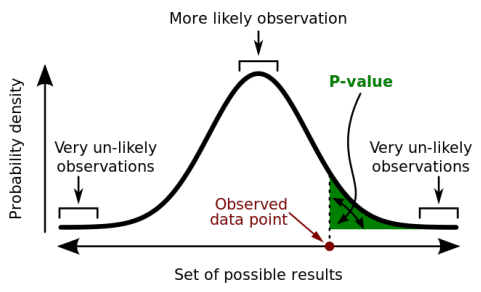
\includegraphics[width=0.5\textwidth]{intro/p-value.png}
\end{center}
\textbf{$\alpha$ level}: A statistical significant p-value is about 0.05. The propability of a type 1 error ($\alpha$) is the probability to reject a true $H_0$. This is inversely proportional to type-II error: to accept a false $H_0$.
\subsection{One-tailed and two-tailed tests}
for two tailed tests sometimes the result needs to be multiplied by 2.
\begin{center}
    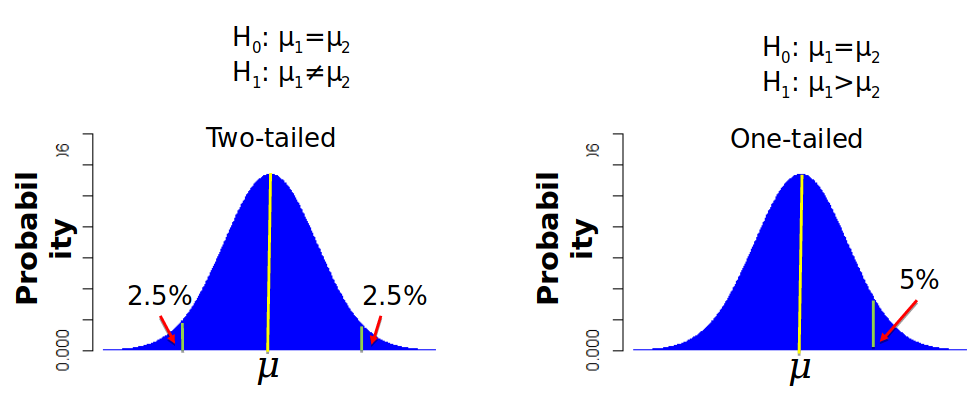
\includegraphics[width = 0.75\textwidth]{intro/tailed-tests.png}
\end{center}
Type I and Type II errors are directly related to false discovery rates (FDR).When multiple tests are used this needs to be corrected for, this is of particular importance in analyses with omics data because $p > n$.\par 
If there are 10 independent tests, each has 5\% probability to be significant when $H-0$ is true (the slide says 'true', but actually false?) ($\alpha = 0.05$). The probability that none is significant is $0.95^{10} = 0.60$, this means that there is a 40\% risk that at least one test will be significant by chance, a type I error. By correcting $\alpha$ to 0.01, the risk of type I error becomes less that 10\%, but we increase the risk of accepting a false $H_0$, type II error.

\subsection{Replicates}
\begin{enumerate}
    \item \textbf{Technical replication:} good to reduce noise (measure the same sample multiple times under the same conditions, reduces measurement error).
    \item \textbf{Biological replication:} good to reduce noise, essential to conclude anything about the general world (naural population) (measure more samples to increase sample size and reduce error).
\end{enumerate}


\subsection{Conclusions from data}
\textbf{natural population}: individuals that can meet and produce viable offspring\\
\textbf{Statistical population}: The entity that your analysis will say something about \\
\textbf{Statistical example}: When we can't measure the whole natural/statistical population, statistics can help draw conclusions from a subsample. 
Error can come from random measurement error, bias (systematic) and contamination (cant be helped by stats).
\subsubsection{Mean}
\begin{itemize}
    \item Arithmetic mean: \\
    population mean: $\mu = \frac{\sum x}{N}$ (actual mean in a full population)\\
    sample mean: $\bar{x} = \frac{\sum x}{n}$ (mean calculated from a statistical sample)
    \item Median: the intermediate rank: (2, 2, 3, \textbf{3}, 3, 3, 5)
    \item Mode: the most likely value: ( four 3's in (3,5,2,3,2,3,3))
\end{itemize}

\subsubsection{Variance}
The variance measures the spread in data ($\sigma ^2$ for the eintire population and $s^2$ for the statistical sample).
$$\sigma^2 = \frac{\sum(x-\mu)^2}{N} \: \: \: \: \: \: \;\;\;\;\;\;\;\; s^2 = \frac{\sum(x - \bar{x})^2}{n-1} $$
the n-1 in the sample variance is a correction factor to account for the error caused by the sample potentially not being representative (can be analytically proven). The standard deviation is the square root of the variance.

\subsubsection{t-test} \label{ttest}
Two sample t-test for independent samples:requires small sample sizes and data that is probably normally distributed. A and B are samples of distinct groups, the test determines whether they doffer statistically significantly or whether the differences are a result of chance.
$$t = \frac{(\bar{x}_{A} - \bar{x}_{B})}{\sqrt{\frac{s_{A}^2}{n_{A}} + \frac{s_{B}^2}{n_{B}}}}$$
t is the difference in population means divided by the difference between individuals within populations. The uncertainty in the estimate of group differences depends on uncertainty in the estimates of group means.\par 
From the result of the t-test the actual p-value can be looked up in a table, it can then be determined whether $H_0$ (the samples are the same and all variation is only a result of chance) is to be accepted or rejected.\\
Degrees of freedom can be calculated by: $$df = n_1 + n_2 -2$$ 
The Standard error of the mean can be calculated by: $$SEM= \frac{s}{\sqrt{n}}= \sqrt{\frac{s^2}{n}}$$
s is the variation in the statistical example(p 118-120 in McKillup).\\
\textbf{The Central Limit Theorem}: Means from repeated samples will be normally distributed and the mean of these means will be a very good approximation of the populaion's true mean value. The standard deviation of this new distribution of means is called the 'STandard error of the mean (SEM)'.\par 
\subsubsection{Hypothesis testing}
The question needs to be specified and from this $H_0$ and $H_1$ need to be determined. Only after this, the experiment should be conducted and the data collected. From this response the correct mathematical distribution and the correct test should be chosen. Based on the statistical analysis (p-values and confidence intervals) the null-hypothesis $H_0$ can be accepted or rejected.\\
\\

\textbf{Example in R: (Lab 1)}
\begin{lstlisting}
males <- rnorm(10, 30, 10) #number of samples, mean, standard deviation
females <- rnorm(10, 30, 10)
t.test(males, females, var.equal = TRUE)
\end{lstlisting}
A t-test can be performed to assess a statistical difference in male and female means. Here, a two-sample t-test for independent samples is used to calculate a p-value. It gives the output:\par
\begin{lstlisting}
	Two Sample t-test

data:  males and females
t = -1.6276, df = 18, p-value = 0.121 #the result is non-significant, p-value > 0.05
#the t-value is the test statistic used to calculate the p-value. It gives the effect size and direction of the effect (+ or -)
alternative hypothesis: true difference in means is not equal to 0
#is not accepted because p-value > 0.05 (the result can happen with 12% probability by pure chance)
95 percent confidence interval:
 -13.835222   1.756148
# the true difference in means is with 95% somewhere in between those values.
sample estimates:
mean of x mean of y 
 29.28238  35.32192 
\end{lstlisting}

This shows no significant difference between the male and female sample, but by pure chance you might get two samples that are significantly different. The experiment is repeated 1000 times, by pure chance some samples should be significantly different: \par
\begin{lstlisting}
P.value <- 1:1000 #create a vector where the p-values are saved
for (i in 1:1000) {
males <- rnorm(10,30,10)
females <- rnorm(10,30,10)
P.value[i] <- t.test(males,females, var.equal=T)$p.value}
sign.tests <-ifelse(P.value <0.05, 1,0) #if the p-value is significant (<0.05), a 1 is added to the vector, otherwise a 0
sum(sign.tests)
\end{lstlisting}

In this case, there were 47 out of 1000 experiments, where the samples were significantly different. This means, the type 1 error rate is 0.047, in 4.7\% of cases the alternative hypothesis is wrongly accepted There should be about $1000\cdot 0.05 = 50$ significant tests on average. If the sample size per test would be larger (here only 10), there would still be about 50 significant tests, becaus the type-I-error rate stays the same. Just the accuracy would improve (for a single t-test, the 95\% confidence interval would be smaller, see output above).\par
But what if there is an actual difference?

\begin{lstlisting}
males <- rnorm(10, 29, 10)
females <- rnorm(10, 30, 10)
t.test(males, females, var.equal = TRUE)
\end{lstlisting}
For only 10 samples, the type-II-error (acceptance of the false null-hypothesis that the samples are not significantly different) will be very large, sampling more will give a better estimate. \textbf{Type-II-errors decrease (and statistical power increases) with the square root of the sample size.}\par 
As discussed above, some samples will have type-I-error when the experiment is conducted often enough, for this reason the analysis needs to be corrected for multiple testing.\par
\begin{lstlisting}
P_value <- 1:(100)
for(i in 1:100){
  males <- rnorm(1000, 30, 10)
  females <- rnorm(1000, 30, 10)
  P_value[i] <- t.test(males, females, var.equal = TRUE)$p.value
}
hist(p.adjust(P_value, "bonferroni")), #ir 'fdr', see below
\end{lstlisting}
The resulting histogram:
\begin{center}
    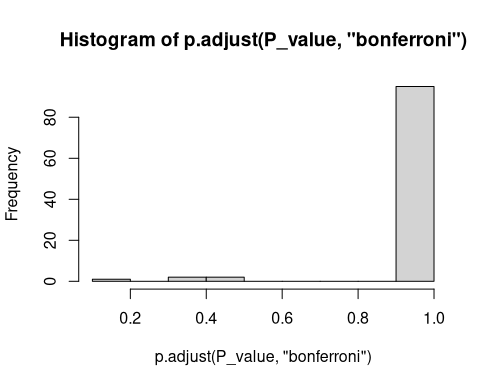
\includegraphics[width = 0.5\textwidth]{lab1/multiple_testing.png}
\end{center}
The \textit{Bonferroni} Method multiplies all p-values with the number of tests conducted, so getting significant results is harder with more test. Another method is the false discovery rate (fdr, aka Benjamini-Hochberg method).\par
Multiple testing in general means that some results that would be significant on their own are discarded because there were multiple tests conducted. For this reason, in biology, sometimes the number of tests are limited beforehand.

\subsection{Different Distributions}

\subsubsection{Standardized normal distribution}
The data is converted to z-scores like this: $$z_{pop} = \frac{(x-\mu)}{\sigma} \: \: \: \: \: \: c z_{sample} = \frac{x-\bar{x}}{s}$$. 
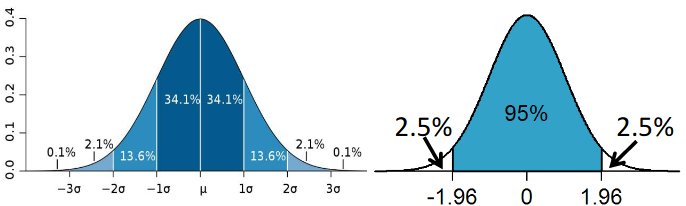
\includegraphics[width = 0.9\textwidth]{intro/normalverteilung2.png}
The area underneath the curve accounts for  100\%, this means all sample values are represented. -1.96$\sigma$ to +1.96$\sigma$ include 95\% of the population (confidence intervall). The formula for the distribution is:
$$Pr(x)_{pop} = \frac{1}{\sigma \sqrt{2 \pi}}\: e^{-\frac{(x-\mu)^2}{2\sigma^2}} \: \: \: \: \: \: \;\;\;\;\;\;\;\ or \: \: \: \: \: \: \;\;\;\;\;\;\;\ Pr(x)_{sample} = \frac{1}{s \sqrt{2 \pi}}\: e^{-\frac{(x-\bar{x})^2}{2 s^2}}$$
Modeled in R by the function \texttt{rnorm(sample size, mean, SD)}.

\subsubsection{Binomial distribution}
A model in which two (binary) outcomes are possible, e.g. Male/Female, Dead/Alive, 1/0.
$$P(x) = \frac{k!}{x!(k-x)!} \times p^x \times q^{(k-x)}$$
P = prob. of x; k = number of samples; x = number of outcome 1; p = $H_0$ prob. of outcome 1; q = $H_0$ prob. of outcome 2. 

\subsubsection{Poisson distribution}
The poisson distribution describes the number of counts when the mean is known ad equals $\bar{x}$, e.g cells in a medium, genes expressed. It assumes that $\lambda = \bar{x} = \sigma^2$ (mean $\approx$ variance)
$$P(x) = e^{-\bar{x}} \times \frac{\bar{x}^x}{x!}$$

\subsubsection{Chi square or $\chi ^2$ distribution}
A squared normal distribution. Widely used in hypothesis testing, it tests for differences in frequencies, goodness of fit of a distribution to a theoretical one or likelihood ration tests. It gives the probability distribution of sums of squares of \textit{k} number of independent normally disributed random variables (its a squared normal distribution).
$$\chi^2 = \sum_{i=1}^{z}\frac{(O_i -E_i)^2}{E_i}$$
E = expected frequency; O = observed frequency; z = number of comparisons; k = degrees of freedom = f(z).

\subsection{Omics data}
Omics Data have their own statistical properties. Intensity Data (e.g fluorescence) should often be log-transformed. Reads are counts, so differential expression may be analyzed in different ways (always including poissin and additional error process, e.g. negative binomial erorrs or poisson-logNormal). R-PAckages that may be used are LIMMA, edgeR or DESeq2.

\subsection{Distributions in R}
R has functions that allow you to sample randomly from distributions (\texttt{rnorm(n, mean, sd)}), or calculate the probability (\texttt{pnorm(q, mean, sd)} with q as a xector of quantiles), the density(\texttt{dnorm(x, mean, sd)} with x as a vector of quantiles), or critical value for a given probability (\texttt{qnorm(p, mean, sd)} with p as a vector of probabilities).\\
\textbf{Simulate a micro-array study on gene expression}\\
Simulate the variability in the data from two independent sources: error of the biological source and of the technical measurement:
\begin{lstlisting}
Bio <- rnorm(1000, 0, 1)
Tech <- rnorm(1000, 0, 2)
Total <- Bio + Tech
\end{lstlisting}
When the sources of the errors are uncorrelated, the variances are additive: $V_{total} = V_{bio} +V_{tech}$
The variance is the square of the standard deviation, so \texttt{var(Total)} should be about 5.\par
The mean expression should be predicted. To calculate this the Standard error of the mean (SEM) can be calculated. $$SEM = \frac{sd}{\sqrt{n}}$$
What happens when you double the amount of technical samples (subjects measuret twice), or when you double the amount of study subjects (more subjects measured)? This can be derived from the formula of the t-test (see section \ref{ttest}). 
$$SE_{total}\: = \:\sqrt{\frac{sd_{bio}^2}{n_{bio}} \: + \: \frac{sd_{tech}^2}{n_{tec}}} $$
\begin{lstlisting}
SE = sqrt(var(Bio)/1000 + var(Tech)/1000)
[1] 0.07061785
#test doubling of samples with the above equation:
sqrt(var(Bio)/1000 + var(Tech)/2000)
[1] 0.0547471
sqrt(var(Bio)/2000 + var(Tech)/2000)
[1] 0.04993436
\end{lstlisting}
It's always better to increase biological replication in terms of statistical power (the precision of the estimate is better). However, the difficulty and effort in doubling the sampling size is not always worth it, and it would be more economic to increase the technical replication.\par
\textbf{What if the data is not normally distributed?} Sometimes log-transforming works well (from poisson to log). If it does not, a generalized linear model should be fitted using a different distribution (poisson or negative binomial)

\subsection{analysis of frequencies in R}
The genotype for a trait is measured in two different populations. Alleles in population 1: 0.40AA, 0.055Aa, 0.05aa. Population 2: 0.80AA, 0.19Aa, 0.01aa. With the Hardy-Weinberg equilibrium (HWE) it can be testet whether there is selection on the locus in each population. The principle states: \textit{allele and genotype frequencies in a population will remain constant from generation to generation in the absence of other evolutionary influences} (wikipedia). $HWE = p^2+2pq+q^2$. These are the expected genotype frequencies with random mating and no selction, and it is tested whether the data deviates from them. We calculate the expected number of genotypes knowing we have sampled 2000 alleles in total from each population.\\
\textbf{Population 1:}\\
calculate the number of alleles
\begin{equation*}
\begin{split}
    A  = & 0.4 \cdot 2 \cdot 1000 + 0.55 \cdot 1000 = 1350  \\
     \Rightarrow& p(A) = 1350/2000 = 0.675\\
    a  =& 2000-1350 = 650 \\
    \Rightarrow& p(a) = 650/2000 = 0.325
\end{split}
\end{equation*}
Exp: $p(A)^2 + 2p(a)P(A) + p(a)^2$ \\
Chi-2: $\frac{(400/456)^2}{456} + \frac{(550-439)^2}{439} + \frac{(50-105)^2}{105} \: = \: 63.8$\\
$P_{HWE}:$
\begin{lstlisting}
1-pchisq(63.8, df = 2)
[1] 1.398881e-14
\end{lstlisting}
The p-value here is very low, the null hypothesis is rejected. There is very strong evidence for selection (or someting else disrupting random association of alleles) in population 1. Population 2 can be tested in the exact same way.\par
Population 1 and 2 can be compared  by reading the observations into a matrix and performin a chi-square test on it (testing that frequencies in each of the matrix's cells are equal).
\begin{lstlisting}
Test.sel<-matrix(rbind(c(400,550,50),c(800,190,10)),2,3)
chisq.test(Test.sel)

Pearsons Chi-squared test
data: Test.sel
X-squared = 335.1351, df = 2, p-value < 2.2e-16
\end{lstlisting}
We reject H0; Selection is acting differently on the locus in population 1 and 2.

\subsection{Residuals}
The residual $\epsilon$ is the difference between the measured y-values and the model's predicted value $\hat{y}$, meaning $\epsilon = y - \hat{y}$. Both the sum and mean of residuals are 0. Plots between observed or predicted y-values and residuals should not show any patterns. Not the data itself should be normally distributed, but the model residuals definitely should. There are different kinds of residuals:
\begin{center}
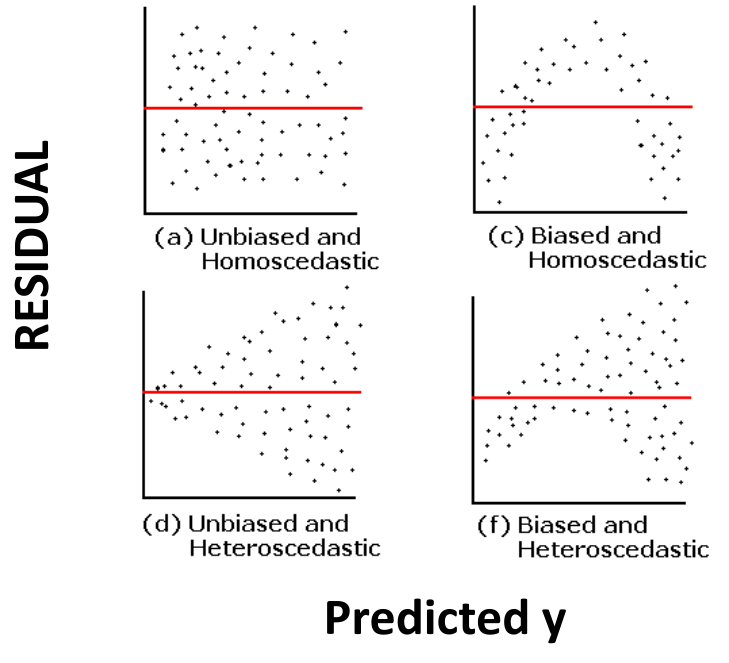
\includegraphics[width = 0.5\textwidth]{intro/residuals.png}
\end{center}

\subsection{Transformation}
Most common transformations:
\begin{itemize}
    \item \textbf{Log}: $x = log_a (x)$ or $log_a(x+1)$ if there are zeros. Log 2 is very common in differential expression analysis $log(A/B) = log(A)-log(B)$
    \item \textbf{square-root}: $x = \sqrt{x}$ or $x = \sqrt{x+0.5}$
    \item \textbf{arcsine}: $x = \arcsin (x)$
\end{itemize}

\subsection{Outliers}
Outliers have a disproportionate effect on model predictions. There are multiple ways of dealing with them:
\begin{itemize}
    \item \textbf{Remove}: If the typo is a mistake in the data, like a typo or if there is an accidental error in the data recording (like the outlier was accidentally recorded from a different population). It is also important for the outlier to be not systematic.
    \item \textbf{Keep, but reduce the influence}: The entire dataset can be transformed to reduce the influence. Robust regressiond and a non-parametric test (using rank rather tan actual value of data-points) can also be used. Robust Regression removes every data point (one by one) and looks how the model changes to give outliers (that strongly change the model) less weight.
    \item \textbf{Change}: Change the value of the outlier toh that of the most extreme observaiton excluding the outlier.
\end{itemize}
It is important to always present both analyses, with and without the outlier. The strategy needs to be always be documented and clearly explained.

\subsection{Statistical significance tests}
Choosing the right test: chapter 23 in MCKillup


\section{ANOVA}
Anova stands for analysis of variances, Chapters 9, 11-15 in McKillup.\par 
It tests for differences between group means, e.g. Gene/Protein expression (both in an exploratory way and as a hypothesis test). It makes several assumptions:
\begin{itemize}
    \item a continuous response
    \item at least one of the explanatory variables is discrete (otherwise regression)
    \item the variance within groups is equal among groups ('Homogenity of variances')
    \item residuals are normally distributed ('assumption of normality')
\end{itemize}
It tests for significance by comparing the variance between individuals within groups to variance among groups (p 140-152 McKillup):
\begin{equation}\label{fvalue}
   \frac{variance \: among \: groups = group+individual+error}{variance\: within\: groups = individual+error}
\end{equation}

\subsection{one-way ANOVA}
\begin{equation*}
    variance_{total} = variance_{within} + variance_{among}
\end{equation*}
If all observations are drawn from the same actual population, then variance between individuals is drawn from the same category. This means it will be equal between individuals from different (assigned) catrgories. Any potential difference between means of the categories is then due to solely individual variation and random sampling.\par 
If the variance between individuals from different categories is much greater than the variance between individuals from the same category, It can be concluded that there is a difference in the means of the categories that contributes to the grater variance.

\subsubsection{Patritioning the sum of squares (SS)}
\begin{itemize}
    \item Total: $SS_T = \sum (x_i - \bar{X})^2$
    \item Between: $SS_M = \sum n_j(\bar{x}_j - \bar{X})$
    \item Within: $SS_i = \sum_j \sum_i (x_{ij} - \bar{x}_j)^2$
\end{itemize}
The total sum of squares is the sum of the SS between groups and the SS within a group (McKillup 141-152).

\subsubsection{Degrees of freedom (df)}
the degrees of freedom describe the numbre of independent observations available for the test. It can be complex to calculate for more complicated designs. \\
\textbf{Example:}
\begin{table}[h]
    \centering
    \begin{tabular}{c|c|c|c|c|c|c|c|c|c|c}
        & \multicolumn{7}{|c|}{samples} & n & $\bar{x}$ & S$^2$\\
        \hline
        \textbf{A} &10 & 24 & 32 & 42 & 32 & 12 & 23 & 7 & 25 & 11.4\\
        \textbf{B} &22 & 43 & 32 & 32 & 44 & 45 &    & 6 & 36.3 & 9.2\\
        \textbf{C} &54 & 34 & 54 & 54 &    &    &    & 4 & 49 & 10 \\
        \hline
        \textbf{Total (T)} &\multicolumn{7}{|c|}{ }& 17 & 34.6 & 13.7\\
    \end{tabular}
\end{table}

\begin{itemize}
    \item Total: $df, SS_T = n_T -1$  ($n_T$ = total number of samples) \\
        $17 - 1 = 16$
    \item Between: $df, SS_M = a-1$ (a = number of groups) \\
        $3 - 1 = 2$
    \item Within: $df, SS_i = n_T -a$ \\
        $17 - 3 = 14$
\end{itemize}

\subsubsection{Variances and F-tests}
The variance is s$^2$.
\begin{itemize}
    \item $s^2 _{between} = \frac{SS_{between}}{df_{between}}$, daraus folgt also: $ \frac{1493}{2} = 746$
    \item $s^2 _{within} = \frac{SS_{within}}{df_{within}} $, daraus folgt also: $ \frac{1507}{14} = 108$
    \item \textbf{calculate F: } $F = \frac{s^2 _{between}}{s^2 _{within}}$, daraus folgt also $\frac{746}{108} = 6.9$
\end{itemize}

\subsubsection{The ANOVA table}
The anova table is the summary of the different group-variations
\begin{table}[h]
    \centering
    \begin{tabular}{c|c|c|c|c}
         \textbf{variation} & \textbf{SS} & \textbf{df} &\textbf{S}$^2$(MS) &\textbf{F}  \\
         \hline
         between & 1493 & 2 & 746 & 6.93 \\
         \hline
         within & 1507 & 14 & 108 & \\
         \hline
         Total & 3000 & 16 && 
    \end{tabular}
\end{table}
Compare the calculated f-Value (see row 'between') for nominator df = 2 and df = 14 (for between and within group): $F_{crit} $ at $ \alpha _{0.05} : \:\: F_{2.14} = 3.74$. The above calculated F is 6.93 > 3.74 which means  $H_0$ (there is no difference between groups) is rejected and the alternative hypothesis is accepted. The rest can be calculated in \textit{R}, the resulting p-value is 0.008

\subsubsection{Post hoc tests}
Which groups differ? With omics data there might be many groups to compare (p>n problem), which makes special strategies necessary.\\
Alternative 1: plot groups with 95\% confidence intervals.\\
Alternative 2: make \textit{planned comparisons} for some group-combinations: A-B, A-C, but not B-C. This requires an a-priori hypothesis for comparison which reduces the number of tests.

\subsubsection{more aspects of ANOVA}
How different groups can be tested against each other with different types of ANOVA:
\begin{figure}[h]
    \centering
    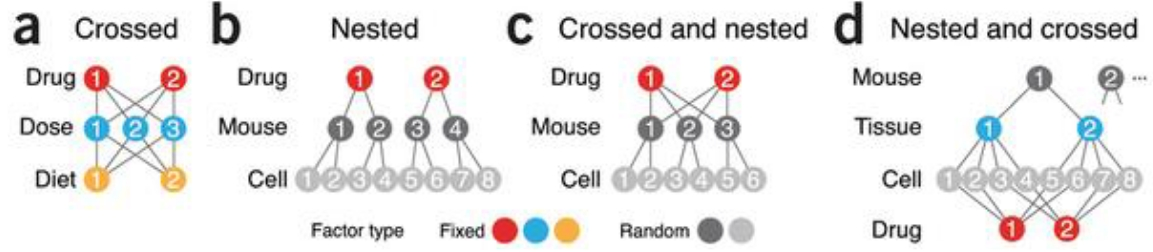
\includegraphics[width = 1\textwidth]{ANOVA/anovakinds.jpg}
\end{figure}

\subsubsection{Example in R for the one-way anova (lab 2)}
Example file that contains the effect of diets A, B, and C on males and females (in weightchange)
\begin{lstlisting}
read.delim("diet.txt")->diet
diet$weight.loss <- diet$pre.weight - diet$weight6weeks #caculate the weight loss and add to the dataset as new variable
boxplot(weight.loss ~ Diet, data = diet, col="light gray", ylab = "Weight loss (kg)", xlab = "Diet type")
abline(h=0,col="blue")
\end{lstlisting}
The data can be visualized in a boxplot, and it seems that diet C has a higher weight loss than the other diets:
\begin{center}
    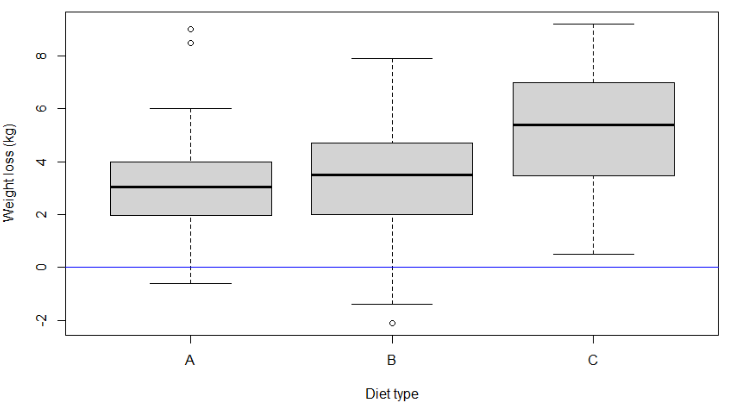
\includegraphics[width = 0.75\textwidth]{lab2/lab2_boxplot.png}
\end{center}
There are two basic ways to perform an ANOVA in R, \texttt{aov()} (analysis of variance, nested designs can be specified) or \texttt{lm()} (linear model, more general and can be used for most types of designs).

\begin{lstlisting}
mod1a <- aov(weight.loss ~ Diet,data=diet)
mod1b <- lm(weight.loss ~ Diet,data=diet)
hist(resid(mod1a))
plot(mod1a)
\end{lstlisting}

\begin{center}
    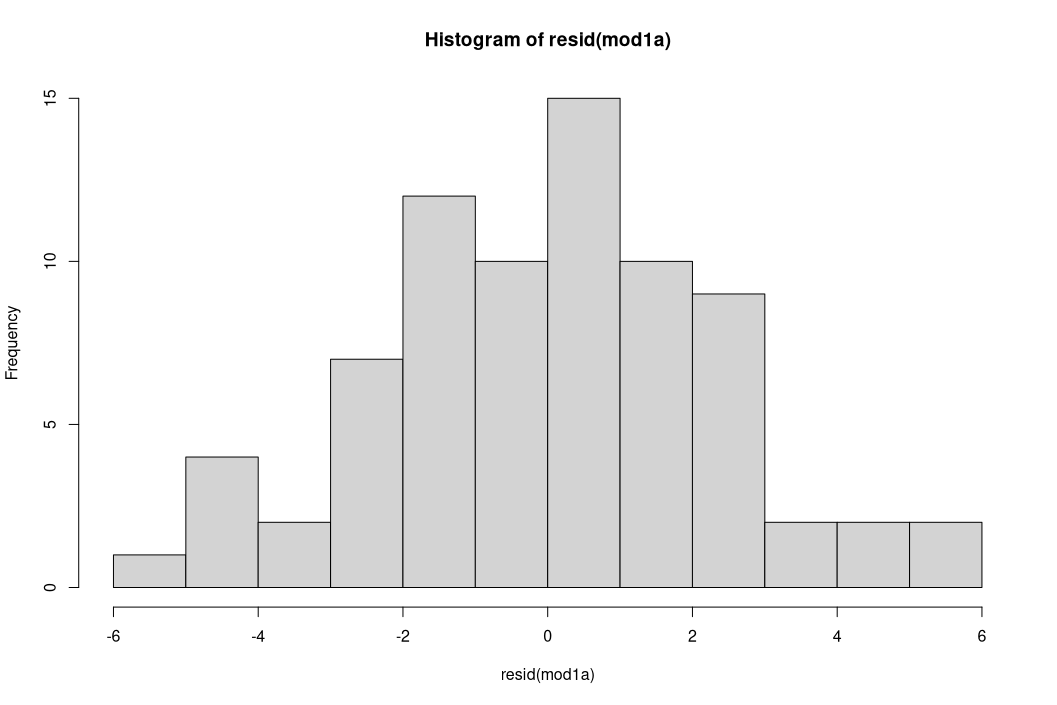
\includegraphics[width = 0.75\textwidth]{lab2/hist_aov_residuals.png}
\end{center}
\begin{center}
    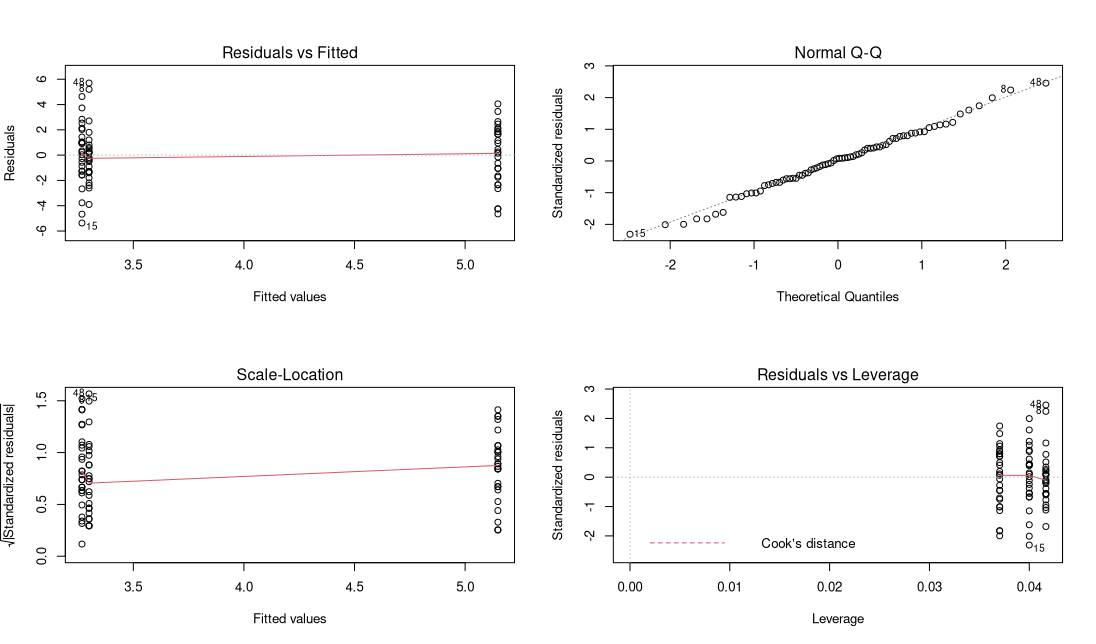
\includegraphics[width = 0.95\textwidth]{lab2/aov_plot.png}
\end{center}
Plots on the left hand side: three columns for Diets A, B, and C (placed on the mean weight loss, not separated by gender) (the standardized residuals are $ \frac{data}{sd(data)}$). If the residuals are normally distributed, the residuals should follow the diagonal line in the QQ-plot pretty closely, as they do here.

\begin{lstlisting}
summary(mod1a)

            Df Sum Sq Mean Sq F value Pr(>F)   
Diet         2   60.5  30.264   5.383 0.0066 **
Residuals   73  410.4   5.622                  
\end{lstlisting}
The F-value is variance among groups divided by variance whithin groups (see equation \ref{fvalue}). Here itmeans that the groups (Diets) seem to be significantly different from one another.

\begin{lstlisting}
summary(mod1b)

Call:
lm(formula = weight.loss ~ Diet, data = diet)

Residuals:
    Min      1Q  Median      3Q     Max 
-5.3680 -1.4420  0.1759  1.6519  5.7000 

Coefficients:
            Estimate Std. Error t value Pr(>|t|)    
(Intercept)   3.3000     0.4840   6.818 2.26e-09 *** # mean weightloss on diet A
#how are diets B and C different from diet A:
DietB        -0.0320     0.6776  -0.047  0.96246    
DietC         1.8481     0.6652   2.778  0.00694 ** #Diet C seems to be significantly different from A (not separated by gender!)

Residual standard error: 2.371 on 73 degrees of freedom
Multiple R-squared:  0.1285,	Adjusted R-squared:  0.1047 
F-statistic: 5.383 on 2 and 73 DF,  p-value: 0.006596
\end{lstlisting}
The diets are ordered alphabetically (as is standard in R) and the first level is taken as the model intercept and its mean value is shown. For diet B and C only the difference to diet A is shown. The R squared value indicates how much of the total individual variation in weight loss is explained by the three diets. The adjusted R-Squared value depends also on the amount of tested criteria (e.g. for more artificial diets with just random weight fluctuation, the adjusted R squared would be lower to compensate for more conditions, in this case the p-value would also be higher).\par 
If you want to compare two models (one with more 'bullshit' variables, one without) you can compare two models with an anova \texttt{anova(mod2a, mod2b, ...)} (more than 2 models can be compared). You can then see which model is the best by the resulting p-value.\par
The F-value is the variance among groups divided by the variance within groups (higher value the more likely it is for the groups to be actually distinct. The p-value describes how likely it is to see this effect by pure chance, it is very low (below 0.05) and therefore significant.\par 
Next, we use the \texttt{Anova()} function (from the \texttt{car} library) to get the anova table with the sum of squares.\\
\begin{lstlisting}
library(car)
Anova(mod1a)

Anova Table (Type II tests)

Response: weight.loss
          Sum Sq Df F value   Pr(>F)   
Diet       60.53  2  5.3831 0.006596 **
Residuals 410.40 73                    


Anova(mod1b)

Anova Table (Type II tests)

Response: weight.loss
          Sum Sq Df F value   Pr(>F)   
Diet       60.53  2  5.3831 0.006596 **
Residuals 410.40 73                    
\end{lstlisting}
For a one-way Anova, the p-values are all the same for type I, II, and III sums of squares, but they often differ for more complex designs. Type I SS are not recommended to test significance, the choice between type II and III depends on your philosophy and the hypothesis tested, in this course we will use type II.\par 

To find out which groups differ, we can perform post hoc tests. One such test is Tukey Honest Significance Differences test.

\begin{lstlisting}
TukeyHSD(mod1a)

  Tukey multiple comparisons of means
    95% family-wise confidence level

Fit: aov(formula = weight.loss ~ Diet, data = diet)

$Diet
         diff        lwr      upr     p adj
B-A -0.032000 -1.6530850 1.589085 0.9987711
C-A  1.848148  0.2567422 3.439554 0.0188047
C-B  1.880148  0.3056826 3.454614 0.0152020


plot(TukeyHSD(mod1a))
\end{lstlisting}
\begin{center}
    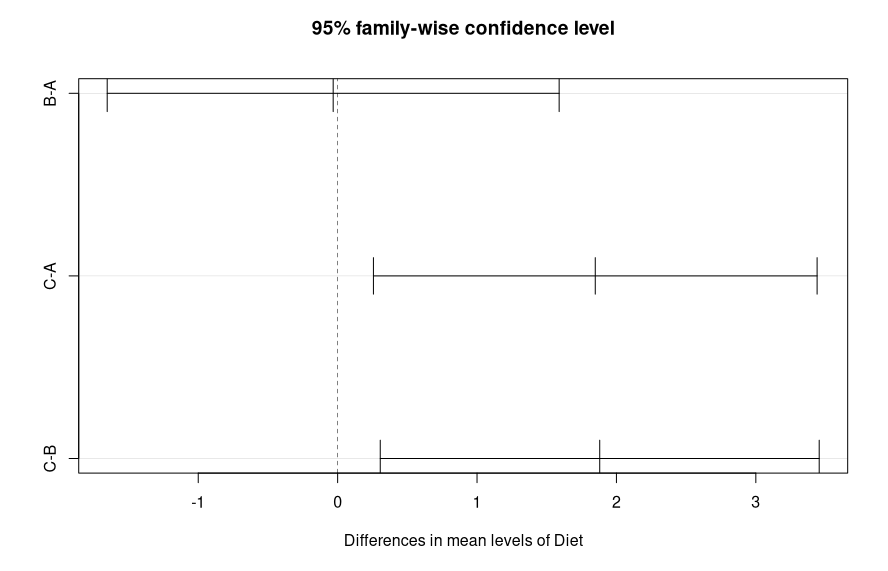
\includegraphics[width = 0.75\textwidth]{lab2/posthoc.png}
\end{center}

How do the diets differ from each other? Diets A and B are very similar to each other and their mean weight loss is about 0. Both diets differ greatly from diet C. The Tukey test tests for pairwise differences, which are given with a 95\% confidence interval.\par 

\subsection{two-way ANOVA}
Multiway ANOVA tests ofr effects of two or more catrgorical factors simltaneously. For a two-way anova there are three effects estimated: factor1, factor 2 and their interaction, some effects may be considered as 'fixed' or 'random', which also affects model estimates and p-values. Simpsons paradox may make it necessary to apply multy way ANOVA to identify actual casual relationships.


\subsubsection{partitioning the sum of squares and y in two-way ANOVA}
The sum of squares and y are different for one-way and tro-way ANOVA.
\renewcommand{\arraystretch}{1.75}
\begin{table}[h]
    \centering
    \begin{tabular}{|c|c|c|}
         \hline
         & \textbf{one-way ANOVA} & \textbf{two-way ANOVA} \\
         \hline
         \textbf{Variance partitioning} & $ SS_{Total} = SS_{within} + SS_{between}$ & $ SS_{Total} = SS_{within} + SS_A + SS_B + SS_{AB}$ \\
         \hline
         \textbf{prediction of y} & $Y_{ji} = \mu + \alpha _j + \epsilon_{ji}$ & $Y_{ijk} = \mu + \alpha _j + \beta_j + (\alpha \beta)_{ij} \epsilon_{ijk}$ \\
         \hline
    \end{tabular}
\end{table}

\subsubsection{ANOVA-designs with dependent observations}
Observations can be dependent or independent, dependent observations have something in common, e.g spatial measures taken from the same patient/tissue/cell culture. There are specific ANOVA-designs for these occasions:
\begin{itemize}
    \item repeated measures ANOVA: within subject, something is measure more than once (e.g. before and afer treatment)
    \item blocked design/nested ANOVA: Accounts for variation between different spatial sampling structures (lanes on a illumina sequencing platform) or hierarchical rlevels (patient/organ/tissue sample)
\end{itemize}

\subsubsection{Fixed or random factors}
\textbf{Fixed factors are decided beforehand}: This is important, they should not be decided after the analysis is carried out to avoid unconscious bias. If the experiment is carried out again, the levels of all factors are the same (like sex, developmental stage, tissue type...). \\
\textbf{Random factors are 'randomly' included in the experiment}: If the experiment is repeated, the levels of the factor will differ (genetic lines in experiment...). The number of lines of the random effect are often directly relates to the number of independent observations in the study.\\
Whether a parameter is fixed or random depends entirely on the experiment and what is to be observed. If a parameter is random or fixed is to be determined before the statistic evaluation, because this desicion can have a great effect on the p-value.


\subsubsection{Example in R (lab 2)}
In more complicated experiments, there are often more explanatory variables, and you have to control for several effects simultaneously in the same model. This is the continuation of the Diet in lab 2, the data of dietary effects on weight loss also include gender.\par

\begin{lstlisting}
mod2a <- lm(weight.loss ~ Diet + gender, data = diet)
summary(mod2a)

Call:
lm(formula = weight.loss ~ Diet + gender, data = diet)

Residuals:
    Min      1Q  Median      3Q     Max 
-5.3262 -1.4018  0.1218  1.6941  5.6445 

Coefficients:
            Estimate Std. Error t value Pr(>|t|)    
(Intercept)  3.26038    0.53890   6.050  5.9e-08 ***
DietB       -0.03422    0.68226  -0.050  0.96014    
DietC        1.84551    0.66982   2.755  0.00742 ** 
genderM      0.09508    0.55258   0.172  0.86387    

Residual standard error: 2.387 on 72 degrees of freedom
Multiple R-squared:  0.1289,	Adjusted R-squared:  0.09259 
F-statistic: 3.551 on 3 and 72 DF,  p-value: 0.01855
\end{lstlisting}
Now, there are the effect of gender and diet in the same model. There are two null-hypotheses now: Men and women loose the same amount of weight, and that all three diets are the same. From the model above we can conclude then there is no significant difference between men and women, $H_0(1)$ is accepted, but there is still a significant difference between diet C and the others, so $H_0(2)$ is rejected.\par
\begin{lstlisting}
plot(mod2a)
\end{lstlisting}
In the plot, there are now six columns on the left hand side for all possible combinations of diet and gender
\begin{center}
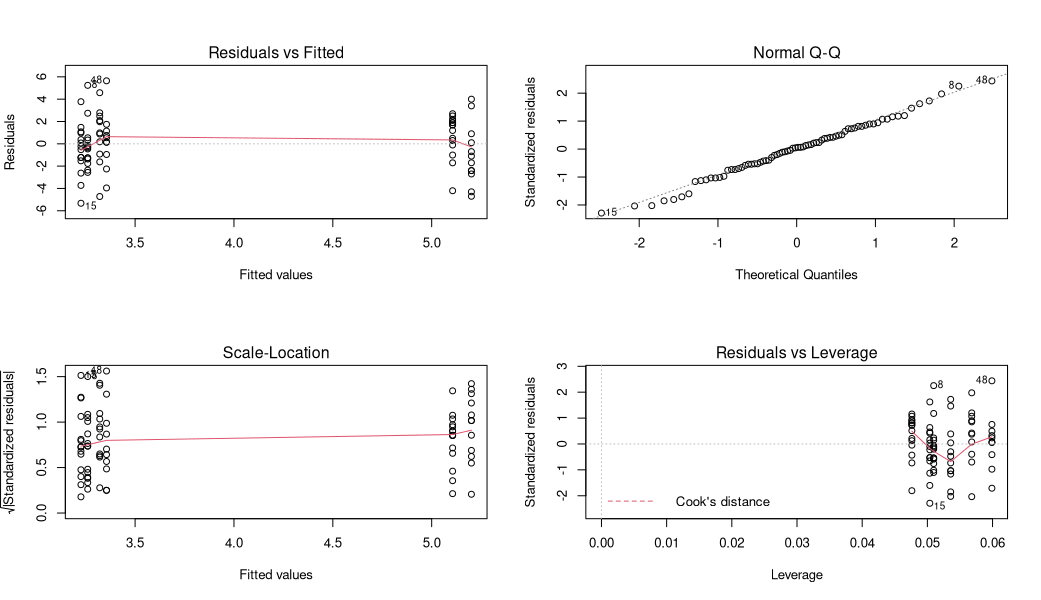
\includegraphics[width = 0.85\textwidth]{lab3/lm_1.png}
\end{center}

However, it is not tested whether men and women respond the same way to all three diets. For this we have to include an interaction between diet and gender. 
\begin{lstlisting}
mod2b <- lm(weight.loss ~ Diet + gender + Diet:gender, data=diet)
mod2c <- lm(weight.loss ~ Diet * gender, data=diet)
#both ways are exactly equivalent
summary(mod2b)

Call:
lm(formula = weight.loss ~ Diet * gender, data = diet)

Residuals:
    Min      1Q  Median      3Q     Max 
-5.5091 -1.2958  0.0705  1.2159  5.4500 

Coefficients:
              Estimate Std. Error t value Pr(>|t|)    
(Intercept)     3.0500     0.6197   4.922 5.49e-06 *** #diet A on females
DietB          -0.4429     0.8764  -0.505   0.6149     #diet B on females
DietC           2.8300     0.8616   3.284   0.0016 **  #diet C on females
genderM         0.6000     0.9600   0.625   0.5340     
DietB:genderM   0.9019     1.3395   0.673   0.5030    
DietC:genderM  -2.2467     1.3145  -1.709   0.0919 .  
Residual standard error: 2.319 on 70 degrees of freedom
Multiple R-squared:  0.2009,	Adjusted R-squared:  0.1438 
F-statistic: 3.519 on 5 and 70 DF,  p-value: 0.006775
\end{lstlisting}
To get the predicted weight loss for males on diet B you have to start from the intercept, add the value for diet B, the value for gender M, and the alue for diet B:gender M, so $3.05 -0.443 +0.60 +0.902 = 4.11$

\begin{lstlisting}
anova(mod2b)

Analysis of Variance Table

Response: weight.loss
            Df Sum Sq Mean Sq F value   Pr(>F)   
Diet         2  60.53 30.2635  5.6292 0.005408 **
gender       1   0.17  0.1687  0.0314 0.859910   
Diet:gender  2  33.90 16.9520  3.1532 0.048842 * 
Residuals   70 376.33  5.3761                    

\end{lstlisting}
There is a third null hypothesis now: men and women respond the same way on all diets. It seems diet C is only significant for women, but men respond to all three diets about the same. There seems to be a significant two-way interaction between diet and gender. Diet C is not generally better, but only for women.\\
s\textbf{plotting the results with lattice and effects}
\begin{lstlisting}
library(lattice)
bwplot(weight.loss ~ Diet|gender, data = diet)
\end{lstlisting}
\begin{center}
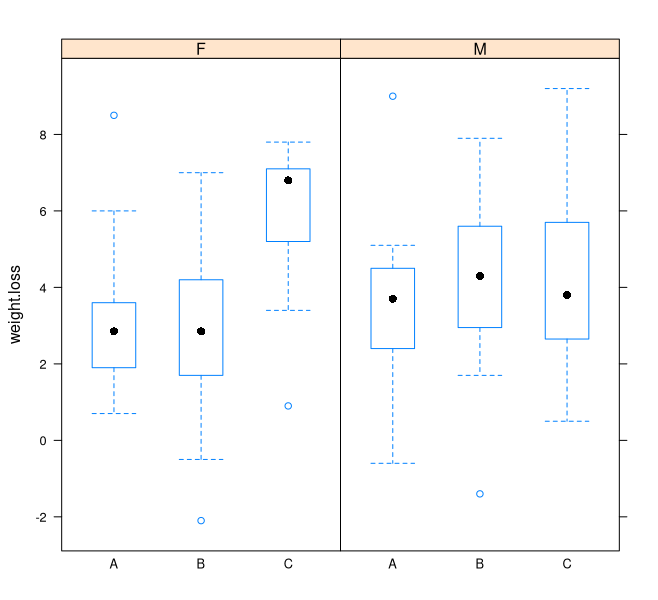
\includegraphics[width = 0.6\textwidth]{lab3/lattice.png}
\end{center}

\begin{lstlisting}
library(effects)
plot(allEffects(mod2b))
\end{lstlisting}
\begin{center}
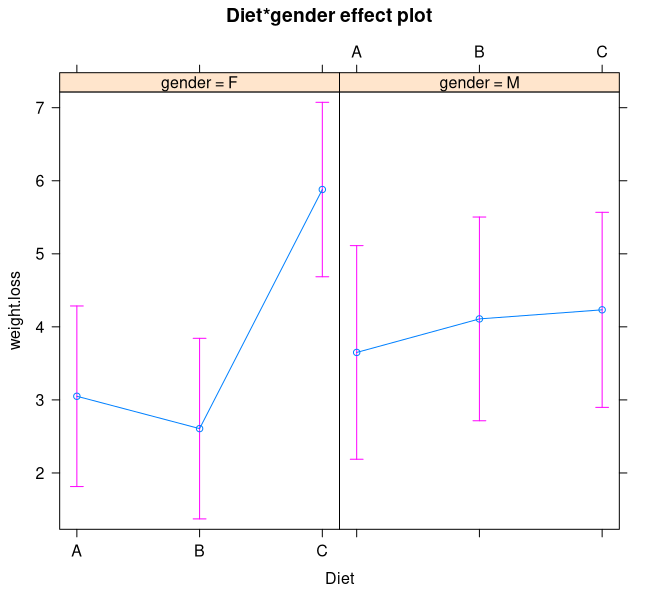
\includegraphics[width = 0.6\textwidth]{lab3/effects.png}
\end{center}

\subsection{calculating the F-ratio}
The F-ratio is: $$F = \frac{Var_{between}}{Var_{within}}$$
The F-Ratio will be calculated for Model I, II and III, with A, B, or their interaction as explanatory variables. MS stands for mean squares and is the variance estimate calculated by $MS = SS/df$.
The standard deviation (error) is equal to the square root of the variance. $\sigma = \sqrt{sd}$
\begin{table}[h]
    \centering
    \begin{tabular}{c|c|c|c}
         explanatory variable & \thead{\textbf{Model I:} \\A and B fixed} & \thead{\textbf{Model II:}\\ A and B random} & \thead{\textbf{Model III:}\\ A fixed, B random} \\
         \hline
         Factor A & $\frac{Factor \: A \: MS}{Error \: MS}$ & $\frac{Factor \: A \: MS}{A \times B \: MS}$ & $\frac{Factor \: A \: MS}{A \times B \: MS}$ \\
         \hline
         Factor B & $\frac{Factor \: B \: MS}{Error \: MS}$ & $\frac{Factor \: B \: MS}{A \times B \: MS}$ & $\frac{Factor \: B \: MS}{Error \: MS}$ \\
         \hline
         Interaction & $\frac{A \times B \: MS}{Error \: MS}$ & $\frac{A \times B \: MS}{Error \: MS}$ & $\frac{A \times B \: MS}{Error \: MS}$ \\
    \end{tabular}
\end{table}
\renewcommand{\arraystretch}{1}

\subsubsection{Generalized linear models (lab 3)}
When data is difficult to transform to a normal distribution, it may be better to model the data using other predefined distributions from generalized linear models. Dummy datasets will be created from binomial and poisson distributions respectively and then analyzed with \texttt{glm()}.

\begin{lstlisting}
#Poisson model:
A <- rpois(10000, 1)
B <- rpois(10000, 1.2) 
pois.data <- data.frame(c(rep("A", 10000), rep("B",10000)), c(A,B))
mod.pois <- glm(pois.data[,2] ~pois.data[,1], family = "poisson")

summary(mod.pois)

Call:
glm(formula = pois.data[, 2] ~ pois.data[, 1], family = "poisson")

Deviance Residuals: 
    Min       1Q   Median       3Q      Max  
-1.5451  -1.4161  -0.1824   0.6722   3.9001  

Coefficients:
                Estimate Std. Error z value Pr(>|z|)    
(Intercept)     0.002696   0.009987    0.27    0.787    
pois.data[, 1]B 0.174278   0.013547   12.87   <2e-16 ***

(Dispersion parameter for poisson family taken to be 1)

    Null deviance: 23388  on 19999  degrees of freedom
Residual deviance: 23222  on 19998  degrees of freedom
AIC: 54353

Number of Fisher Scoring iterations: 5
\end{lstlisting}

The data is usually transformed (often logarithmic) when a general linear model is used. Therefore, the coefficients are not straightforward to understand and may need to be back-transformed to make sense. in this case the estimate can be back transformed by exponentiating, exp(Std. error) gives the standard deviation entered in the beginning (nit exactly since this is a random process).

\begin{lstlisting}
#binomial model

A <- rbinom(10000, 1, 0.2)
B <- rbinom(10000, 1, 0.1)
binom.data <- data.frame(c(rep('A', 10000), rep('B', 10000)), c(A,B))
mod.binom <- glm(binom.data[,2]~binom.data[,1], family = 'binomial')
summary(mod.binom)

Call:
glm(formula = binom.data[, 2] ~ binom.data[, 1], family = "binomial")

Deviance Residuals: 
    Min       1Q   Median       3Q      Max  
-0.6665  -0.6665  -0.4646  -0.4646   2.1353  

Coefficients:
                 Estimate Std. Error z value Pr(>|z|)    
(Intercept)      -1.39130    0.02504  -55.57   <2e-16 ***
binom.data[, 1]B -0.78062    0.04142  -18.85   <2e-16 ***

(Dispersion parameter for binomial family taken to be 1)

    Null deviance: 16960  on 19999  degrees of freedom
Residual deviance: 16588  on 19998  degrees of freedom
AIC: 16592

Number of Fisher Scoring iterations: 4


Anova(mod.binom)

Analysis of Deviance Table (Type II tests)

Response: binom.data[, 2]
                LR Chisq Df Pr(>Chisq)    
binom.data[, 1]   372.34  1  < 2.2e-16 ***

\end{lstlisting}

A binomial distribution is transormed as log(p/(1-p)), the standard errors can be back-transformed by $\frac{e^{-1.39}}{1+e^{-1.39}} = 0.198$, again the deviation comes from rounding errors. 

\subsection{Linear mixed effect models (LMEs) (lab 2 ex. 4)}
This is explained practically in R, using the Jimsonweed Dataset, it contains the length/width (LenWid) ratio of two types of leaves (G and N). Three seeds of each type were planted in 16 pots (Pot is the pot identification number (as factor here).\par 
The first analysis of variance will be conducted with 'pot' as a fixed factor (this means the seeds/plants are considered as experimental units representing the true value of replication of the effect of weed 'type').

\begin{lstlisting}
read.delim("jimson.txt") -> dat#
fm1a <- aov(LenWid ~ Type * Pot, data = dat)
summary(fm1a)
            Df Sum Sq Mean Sq F value   Pr(>F)    
Type         1  7.321   7.321 412.575  < 2e-16 ***
Pot         15  0.898   0.060   3.373 0.000342 ***
Type:Pot    15  0.305   0.020   1.146 0.336418    
Residuals   64  1.136   0.018 
\end{lstlisting}

The analysis can also be performed with 'pot' as a random effect (the pots are considered randomly selected experimental units representing the true level of replication of the effect of weed 'type')

\begin{lstlisting}
fm1b <- aov(LenWid ~ Type + Error(Pot + Type:Pot), data = dat)
summary(fm1b)

Error: Pot
          Df Sum Sq Mean Sq F value Pr(>F)
Residuals 15 0.8977 0.05985               

Error: Pot:Type
          Df Sum Sq Mean Sq F value   Pr(>F)    
Type       1  7.321   7.321     360 6.76e-12 ***
Residuals 15  0.305   0.020                     
Error: Within
          Df Sum Sq Mean Sq F value Pr(>F)
Residuals 64  1.136 0.01774      
\end{lstlisting}

The two models use different error variances and degrees of freedom for calculating the p-value. Still, both models are significant since there were a lot of different pots used. With less pots the species of plant might have been less significant than the choice of pot. This can be caused by slightly different conditions between the pots, but also by chance. The effect can be minimized by using many pots.\par 
To better understand this effect the dataset will be reduced to only the first two pots, first the pot as a fixed effect:

\begin{lstlisting}
dat2 <- subset(dat, (Pot=="16533") | (Pot=="16534"))
fm2a <- aov(LenWid ~ Type + Pot + Type:Pot, data=dat2)
summary(fm2a)
            Df Sum Sq Mean Sq F value   Pr(>F)    
Type         1 0.9352  0.9352 117.636 4.61e-06 ***
Pot          1 0.0114  0.0114   1.435    0.265    
Type:Pot     1 0.0200  0.0200   2.517    0.151    
Residuals    8 0.0636  0.0080   
\end{lstlisting}

The number of observations are considered as each seed, whether the effect is different on the two pots is not considered. The F-values are calculated then as: (Type SS)/(residual SS) (with number of DFs ~ sumber of seeds.
Then, the pot as a random effect:

\begin{lstlisting}
fm2b <- aov(LenWid ~ Type + Error(Pot+ Type:Pot), data=dat2)
summary(fm2b)
Error: Pot
          Df  Sum Sq Mean Sq F value Pr(>F)
Residuals  1 0.01141 0.01141               

Error: Pot:Type
          Df Sum Sq Mean Sq F value Pr(>F)  
Type       1 0.9352  0.9352   46.74 0.0925 .
Residuals  1 0.0200  0.0200                 
---
Error: Within
          Df Sum Sq Mean Sq F value Pr(>F)
Residuals  8 0.0636 0.00795 
\end{lstlisting}

The error term is defined as the variance in the effect (difference between types) among the two pots. The F-ratio is: (Type SS)/(pot:Type SS) with only one (2-1) degree of freedom (DF).\par 
In this case including 'pot' as a random factor is probably correct, because the difference between types in general is of interest, not the correlation between difference in types and difference in pots (assuming there were the same experimental conditions for all this). If there are only two pots, it is hard to tell whether they actually differ or not due to the small sample size (in a good experiment you would plan to have pot as a random variable beforehand and then use enough pots).\par 
This is applied when an experiment is repeated, the repetitions are interpreted as a random effect, just as different pots. Usually, a minimum of 6 levels is a rule for analyzing factors as random.

\begin{lstlisting}
library(lattice)
bwplot(LenWid ~ Type|Pot, data = dat)
\end{lstlisting}

\begin{center}
    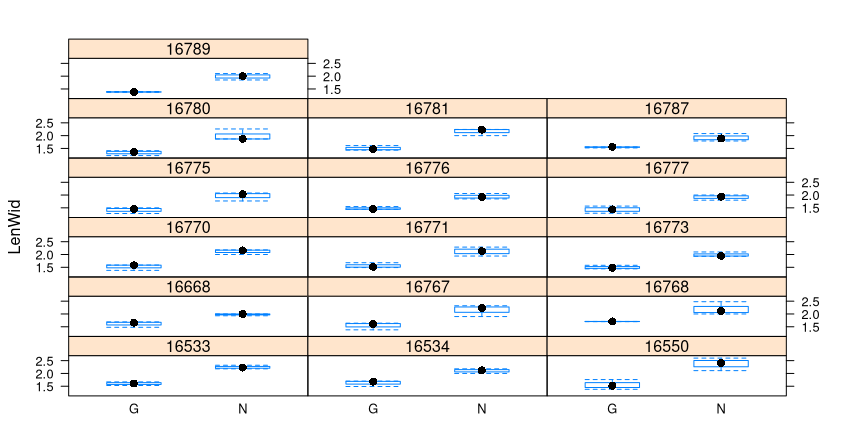
\includegraphics[width = 0.75\textwidth]{lab2/ex4.png}
\end{center}

\subsection{correlation and regression (lab 3)}

\subsubsection{Correlation}
The correlation coefficient gives the amount of covariance between a pair of continuous variables relative to the normal amount of variance in the variables. This will be illustratedby simulating two traits using the \texttt{rnorm()} function, which are (genetically) correlated due to sharing some of their underlying genes. The traits also vary independently from each other because some of their genes are private and affect one but not the other trait. There is also envireonmental variance (measurenment error), that affects both traits but independently.\par 
Two datasets, A and B, will be created as described above. The phenotypic variation among study subjects come from both the genes that are shared and the private ones. Also the measurenment error affects both traits independently.

\begin{lstlisting}
shared <- rnorm(1000, 0, 20) #standard deviation = 10 -> variance = 10^2
private.A <- rnorm(1000, 0, 20)
private.B <- rnorm(1000, 0, 20)
env.A <- rnorm(1000, 0, 10)
env.B <- rnorm(1000, 0, 10)
\end{lstlisting}
\noindent
The variance is additive, this makes the following operation possible which combines the datasets into A and B:

\begin{lstlisting}
A <- shared +private.A +env.A
B <- shared + private.B +env.B
\end{lstlisting}
The true correlation coefficient $\rho$ can be calculated as follows: $$\rho = \frac{cov(A, B)}{sd(A) \cdot sd(B)} \;\; , \;\;\; \sqrt{sd} = var$$
Variances are additive, which means that \texttt{var(A) = var(shared) + var(private.A) + var(env.A)} (and the same goes for B). The covariance between A and B comes only from one shared component, which means \texttt{var(shared) = cov(shared, shared)}. This is equal to the covariance between A and B, because there is no covariance between A and B from the provate genes or the environment (by definition)
\begin{lstlisting}
rho = cov(A, B)/(sqrt(var(A))*sqrt(var(B)))
     > rho = 0.4642041
     > cor(A, B) = 0.4642041 
\end{lstlisting}

\texttt{cor(A, B) }gives the same value because it is applied to the same data, \texttt{cor.test(A, B)} should be used.

\begin{lstlisting}
cor.test(A,B)

	Pearson's product-moment correlation

data:  A and B
t = 16.557, df = 998, p-value < 2.2e-16
alternative hypothesis: true correlation is not equal to 0
95 percent confidence interval:
 0.4141286 0.5114782
sample estimates:
      cor 
0.4642041  
\end{lstlisting}

The 95\% confidence interval includes the correlation above. (they should not be exactly the same but here they somehow are?)

\subsubsection{simple linear regression}
For this, the american crime dataset will be used again, first only looking at violent crime and police funding. It does not seem like there could be an unidirectional casual relationship between the two variables, which would make correlation (as opposed to regression) the better method. The next step is to find the dependent variable (f(x) to the independent variable x), but in cases like this there is no definitive answer, the hypothesis decides. Predicting how differences in police funding affect crime (and thus finding a way to minimize crime through correct police funding). The regression slope describes a quantifiable change in y (f(x)) with a change in x. The model should be plotted before the results are evaluated.

\begin{lstlisting}
simple.1a <- lm(violent.crime ~ police.funding, data = crime)
par(mfrow=c(2,2)) 
plot(simple.1a)
\end{lstlisting}

\begin{center}
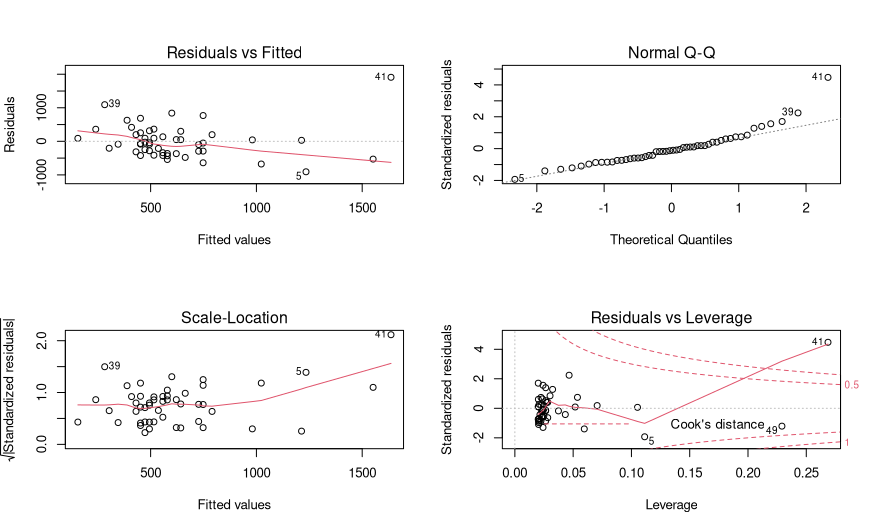
\includegraphics[width = 0.85\textwidth]{lab3/plot-vcrime-vs-police.png}
\end{center}


For regression the bottom right plot is the most important.\par 
Point 41 seems to be an outlier, it has a way bigger crime rate than any other point. It is outside cook's distance, which means it also has a very high leverage. The influence of the outlier needs to be reduced to get a good model. It can either be removed (which is a legitimate choice in this case, because the points makes the model significant and removing it would be conservative), or the data can be log-transformed.

\begin{lstlisting}
simple.1b <- lm(log10(violent.crime) ~ police.funding, data = crime)
summary(simple.1b)

Residuals:
    Min      1Q  Median      3Q     Max 
-1.0839 -0.2538  0.0644  0.2800  0.6736 

Coefficients:
               Estimate Std. Error t value Pr(>|t|)    
(Intercept)    2.240170   0.163432  13.707   <2e-16 ***
police.funding 0.010206   0.004069   2.508   0.0156 *  #the mnodel was made less significant by removing the influence of the outlier 

Residual standard error: 0.3937 on 48 degrees of freedom
Multiple R-squared:  0.1159,	Adjusted R-squared:  0.09744 
F-statistic:  6.29 on 1 and 48 DF,  p-value: 0.01558
\end{lstlisting}

There is a weak but positive relationship between police funding and crime rate. Cities with problems need to invest more in police, but the relationship is not so strong because investing more should hopefully decrease crime. The regression coefficient (0.010206) is the 'slope', one unit change in police funding changes 0.01 unit in crime. \par 
The p-value is calculated by the t-statistic, but it can also be derived from the F-statistics in the model by \texttt{Anova()} (in this specific case the p-value and F-statistic for the total model is the same as for police funding, because it was the only variable included in the model).\par 
the adjusted R squared value can be understood by introducing 'bullshit' variables into the model:

\begin{lstlisting}
number.of.oranges <-rnorm(length(crime$violent.crime), 100, 10)
number.of.apples <- rnorm(length(crime$violent.crime), 100, 10)

mod2a <-lm(log10(violent.crime)~police.funding, data = crime)
summary(mod2a)
Residuals:
    Min      1Q  Median      3Q     Max 
-1.0839 -0.2538  0.0644  0.2800  0.6736 

Coefficients:
               Estimate Std. Error t value Pr(>|t|)    
(Intercept)    2.240170   0.163432  13.707   <2e-16 ***
police.funding 0.010206   0.004069   2.508   0.0156 *  

Residual standard error: 0.3937 on 48 degrees of freedom
Multiple R-squared:  0.1159,	Adjusted R-squared:  0.09744 ##
F-statistic:  6.29 on 1 and 48 DF,  p-value: 0.01558

mod2b <- lm(log10(violent.crime)~ police.funding+number.of.oranges+number.of.apples, data = crime)
summary(mod2b)
Residuals:
     Min       1Q   Median       3Q      Max 
-1.08699 -0.23018  0.08349  0.25198  0.70203 

Coefficients:
                   Estimate Std. Error t value Pr(>|t|)  
(Intercept)        2.033608   0.829384   2.452   0.0181 *
police.funding     0.010151   0.004207   2.413   0.0199 *
number.of.oranges -0.001284   0.005075  -0.253   0.8014  
number.of.apples   0.003354   0.005838   0.575   0.5684  

Residual standard error: 0.4002 on 46 degrees of freedom
Multiple R-squared:  0.1243,	Adjusted R-squared:  0.06722 #the adjusted p-squared is lower than before
F-statistic: 2.177 on 3 and 46 DF,  p-value: 0.1035 
\end{lstlisting}

None of the 'bullshit' variables are significantly related. The two models can be compared by \texttt{anova(mod2a, mod2b)}. The p-value tells you whether the 'bullshit' model explained significantly more of the variation in crime.

\subsubsection{robust regression}
If the data can't be log-transformed to remove the outlier, robust regression can also be applied, in this case with the \texttt{MASS} package.

\begin{lstlisting}
library(MASS)
simple.3 <- rlm(violent.crime~police.funding, data = crime)

summary(simple.3)
Residuals:
    Min      1Q  Median      3Q     Max 
-597.48 -296.20  -35.56  263.44 2381.51 

Coefficients:
               Value    Std. Error t value 
(Intercept)     81.6553 166.9926     0.4890
police.funding  12.5794   4.1580     3.0254

Residual standard error: 427.6 on 48 degrees of freedom

Anova(simple.3)
Analysis of Deviance Table (Type II tests)

Response: violent.crime
               Df     F   Pr(>F)   
police.funding  1 9.153 0.003982 **
Residuals      48  
\end{lstlisting}

The robust regression reduced the influence of the outlier \texttt{plot(simple.3)}.\par 
The untransformed model has the highest p-value due to point 41. Log transforming reduced its influence but may have removed the data further from a normal distribution (bad). Robust regression is ok here if all other assumptions of normality are fulfilled. The robust regression gives a statistical significance somewhere between the other two models before and predicts a weaker relationship than the standard simple regression. In this example, this approach is the best. One outlier still has a little to much influence, but if the chioce is sufficiently motivated it could be removed (when still showing the manipulated tata next to the raw data).

\subsubsection{multiple linear regression}

Look at all five variables of the american crime dataset. In this case, school attendance is the independent variable (x) and crime ist the independent variable (f(x)), because it again makes sense to want to predict crime based on other factors it may depend on. the dataset can be plotted in its entirety (\texttt{plot(crime)}). For the correlation matrix see chapter \ref{crimecorrmatrix}.\par 
It can be observed that the two variables describing crime are highly correlated. The new variables added (education) are onl weakly negatively correlated to crime. Multiple regression will be used to solve the problem that the education variables are also correlated with each other.\par
Given that the crime variables and education variables are highly correlated among each other, it may be useful to just analyze one of each together with police funding.

First, two seperate simple regressions will be performed for each explanatory variable on its effect on violent crime, and then the output of that will be compared to a multiple regression including both.

\begin{lstlisting}
uni.1a <- lm(log10(violent.crime) ~ police.funding, data = crime)
summary(uni.1a)
Residuals:
    Min      1Q  Median      3Q     Max 
-1.0839 -0.2538  0.0644  0.2800  0.6736 

Coefficients:
               Estimate Std. Error t value Pr(>|t|)    
(Intercept)    2.240170   0.163432  13.707   <2e-16 ***
police.funding 0.010206   0.004069   2.508   0.0156 *  

Residual standard error: 0.3937 on 48 degrees of freedom
Multiple R-squared:  0.1159,	Adjusted R-squared:  0.09744 
F-statistic:  6.29 on 1 and 48 DF,  p-value: 0.01558


uni.1b <- lm(log10(violent.crime) ~ perc.highschool, data = crime)
summary(uni.1b)
Residuals:
     Min       1Q   Median       3Q      Max 
-1.08368 -0.16877  0.04738  0.26701  0.96509 

Coefficients:
                Estimate Std. Error t value Pr(>|t|)    
(Intercept)      3.37915    0.34042   9.926 3.23e-13 ***
perc.highschool -0.01282    0.00571  -2.245   0.0294 *  

Residual standard error: 0.3983 on 48 degrees of freedom
Multiple R-squared:  0.095,	Adjusted R-squared:  0.07614 
F-statistic: 5.039 on 1 and 48 DF,  p-value: 0.02943
\end{lstlisting}
The correlation of the explanatory variables by themselves is slightly significant (note the estimates, positive correlation for police funding, negative for highschool education).

\begin{lstlisting}
multi.1 <- lm(log10(violent.crime) ~ police.funding + perc.highschool, data = crime)
summary(multi.1)
Residuals:
     Min       1Q   Median       3Q      Max 
-0.98269 -0.20166  0.04773  0.26147  0.56757 

Coefficients:
                 Estimate Std. Error t value Pr(>|t|)    
(Intercept)      3.058161   0.333139   9.180  4.7e-12 ***
police.funding   0.011483   0.003842   2.989  0.00444 ** 
perc.highschool -0.014732   0.005328  -2.765  0.00811 ** 

Residual standard error: 0.369 on 47 degrees of freedom
Multiple R-squared:  0.2396,	Adjusted R-squared:  0.2072 
F-statistic: 7.403 on 2 and 47 DF,  p-value: 0.001603
\end{lstlisting}

The p value for both variables becomes more significant in multiple refression. This will be the case when both explanatory variables explain variation in y and they are not very correlated to each other. This is because the p-values are calculated as the amount of variation in y explained by x$_1$ and x$_2$ respectively, relative to the amount of residual variation not explained by the model. This latter variation decreases when we add both varables to the model. \par 
The increased significance is not an effect of this. For example, when two variables are highly correlated to each other, then one variable might lose its significance when both are added to the model, because the model judges that it is only one of the variables that is actually linked to the y-variable. Technically this happens because thaddition of another variable in this case does not lead to more variation in y being explained (SSR), so the variation explained by this added variable is very small and the residual variation (SSE) stays about the same.\par 
Visualizing relationships between more than 2 variables quickly becomes difficult (multivariante techniques). The variables can be plotted in R:

\begin{lstlisting}
library(scatterplot3d)
scatterplot3d(crime$police.funding, crime$perc.highschool, crime$violent.crime, pch=20)
\end{lstlisting}

There are problems when we try to use all four variables at once: 
\begin{lstlisting}
multi.2 <- lm(log10(violent.crime) ~ crime.rate + police.funding + perc.highschool + perc.college, data = crime)
summary(multi.2)

Residuals:
     Min       1Q   Median       3Q      Max 
-0.82198 -0.16288  0.01992  0.17903  0.57435 

Coefficients:
                  Estimate Std. Error t value Pr(>|t|)    
(Intercept)      2.6775734  0.3028133   8.842 2.12e-11 ***
crime.rate       0.0008489  0.0001757   4.830 1.62e-05 ***
police.funding   0.0010948  0.0037215   0.294  0.76997    
perc.highschool -0.0166471  0.0059599  -2.793  0.00764 ** 
perc.college     0.0199717  0.0112606   1.774  0.08290 .  

Residual standard error: 0.2964 on 45 degrees of freedom
Multiple R-squared:  0.5301,	Adjusted R-squared:  0.4883 
F-statistic: 12.69 on 4 and 45 DF,  p-value: 5.4e-07
\end{lstlisting}

Police funding seems to be no longer significant.\par 
The colinearity between the two crime variables (one as dependent/response and one as independent/explanatory) caused problems. The crime rate is highly correlated with violent crime, which means it explains that data way better than the police funding. \par
When there are several highly correlated variables in a dataset, the model might have problems, this still holds when we leave out the crime.rate statistic.

\begin{lstlisting}
multi.3 <- lm(log(violent.crime) ~ police.funding + perc.highschool + perc.college, data = crime)
summary(multi.3)

Residuals:
     Min       1Q   Median       3Q      Max 
-1.99626 -0.54942  0.06979  0.61166  1.44817 

Coefficients:
                 Estimate Std. Error t value Pr(>|t|)    
(Intercept)      7.444773   0.786091   9.471 2.23e-12 ***
police.funding   0.025558   0.008677   2.946  0.00504 ** 
perc.highschool -0.053087   0.016306  -3.256  0.00213 ** 
perc.college     0.054791   0.031523   1.738  0.08888 .  

Residual standard error: 0.8319 on 46 degrees of freedom
Multiple R-squared:  0.2864,	Adjusted R-squared:  0.2399 
F-statistic: 6.155 on 3 and 46 DF,  p-value: 0.001315
\end{lstlisting}

Here there are again problems, the model predicted that college attendance seems to be slightly positively correlated to crime.
The correlation matrix can be compared to the partial correlation matrices of the other 5 variables by using the \texttt{RcmdrMisc} package and running \texttt{partial.cor(crime)}.\par 
Ideally both crime variables weould be the response with the other three as explanatory.

\section{PCA and Multivariante hypothesis testing}
Chapter 22 in McKillup. in bioinformatics mostly used to analyze and visualize the relationships between thousands of genes, transcripts and proteins, metabolites etc. It helps detecting differences between groups of individuals soch as populations or different treatments without defining those groups a priori. It does that by creating latent, uncorrelated variables (principal components, PCs) from a large number of correlated variables to describe their variation. \\
Multivariante Data means that a single sample is measured for several responses. Multivariante methods can be used to test hypotheses involving more than one response variable and see groups in patterns and data.\par 

\subsection{Matrices describing relationships between variables}
Variance covariance matrix C and correlation matrix R:
\begin{equation*} 
C \: = \:
    \begin{pmatrix}
    var_1 & cov_{1,2} & cov_{1,3} & cov_{1,4} \\
    cov_{2,1} & var_2 & cov_{2,3} & cov_{2,4} \\
    cov_{3,1} & cov_{3,2} & var_3 & cov_{3,4} \\
    cov_{4,1} & cov_{4,2} & cov_{4,3} & var_4
    \end{pmatrix}
; \; \; \; \; R \:=\:
    \begin{pmatrix}
    r & r_{1,2} & r_{1,3} & r_{1,4} \\
    r_{2,1} & r & r_{2,3} & r_{2,4} \\
    r_{3,1} & r_{3,2} & r & r_{3,4} \\
    r_{4,1} & r_{4,2} & r_{4,3} & r
    \end{pmatrix}
\end{equation*}
C or R can be used to extract a new set of a lower number of derived variables (latent variables), that are easier to grasp than the original variables. The derived variables are all linear combinations of the original variables such that : $Z = c_1X_1 + c_2X_2 + c_3X_3 + c_4X_4 + k$.\par 
On a practical example: $X_1, X_2, X_3, X_4$ are categories, each with multiple observations (e.g. height, weight, body fat percentage, hair color of the same person) are to be derived to $Z_1, Z_2$ (constructed differently depending on the specific method). Each new derived variable is associated with an \textit{eigenvlaue} $\lambda$, which describes the amount of variance in  the original data matrix that is explained by a given variable. \par 
Each derived variable is also associated with an \textit{eigenvector}, the set of coefficients that describes the loading that each original variable has on the derived variable. It is often standardized to correlation coefficients.
\begin{table}[h]
    \centering
    \begin{tabular}{c c c}
         & $Z_1$ & $Z_2$ \\
         & & \\
         $X_1$ & \multicolumn{2}{c}{\multirow{4}{*}{$\begin{pmatrix}
                                                    c_{1,1} & c_{2,1}\\
                                                    c_{1,2} & c_{2,2}\\
                                                    c_{1,3} & c_{2,3}\\
                                                    c_{1,4} & c_{2,4}\\
                                                    \end{pmatrix}$}}\\
         $X_2$ & \multicolumn{2}{c}{}\\
         $X_3$ & \multicolumn{2}{c}{}\\
         $X_4$ & \multicolumn{2}{c}{}\\
    \end{tabular}
\end{table}
\subsection{Principal component analysis}
The original data set $X_{1:p}$ is too big to make sense of. With principal component analysis on the variables of $X_{1:p}$ to get to a new set of $Z_{1:k}$ derived variables, where $k << p$ that are called principal components. This Method is very frequently used in ecology and evolution to characterize patterns of variation/covariation among a set of variables, when there are 'too many' explanatory variables relative to our sample size, or to classify samples/observations in fewer dimenstions than our original variables.\\
\textbf{Redundancy:}
\begin{center}
    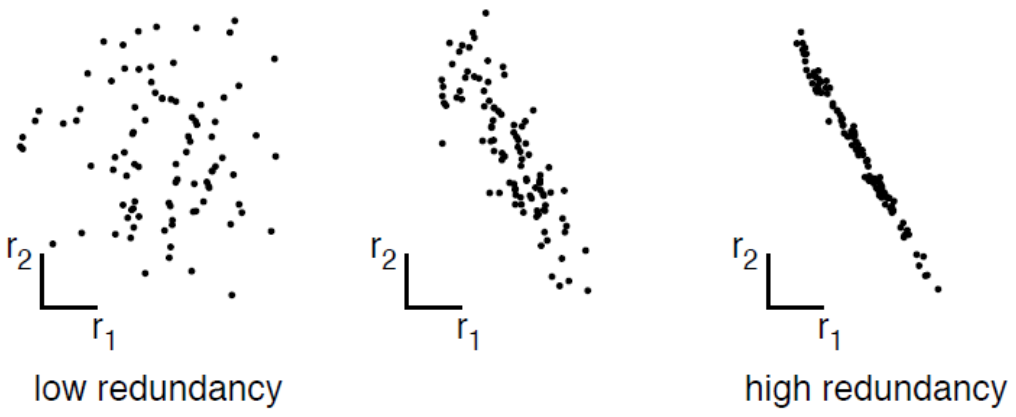
\includegraphics[width = 0.6\textwidth]{PCA/pca_redundancy.png}
\end{center}
Principal components are orthogonal (uncorrelated to each other) by default. The PCA is usually based on a correlation matrix (recommended in most cases, because some components might not be orthogonal using the covariance matrix).

\begin{figure}
\begin{center}
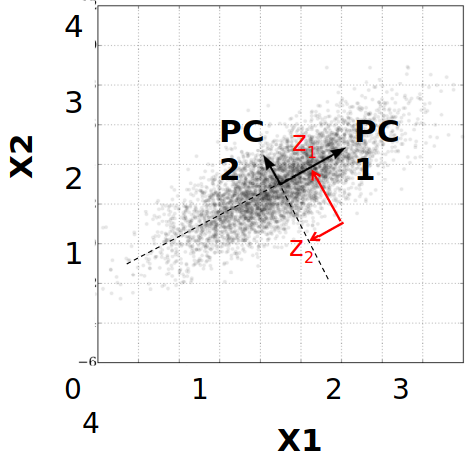
\includegraphics[width = 0.4\textwidth]{PCA/PCA_components.png}
\end{center}
\end{figure}

\begin{align*}
    PC_1: \;\;	\frac{1.2}{1.2+0.1} = 0.92	\; \; \; \; & \Rightarrow \; \; \;\; \lambda_{PC1} = 1.2 \\
	PC_2: \;\;	\frac{0.1}{1.2+0.1} = 0.08  \; \; \; \; & \Rightarrow \;\; \; \; \lambda_{PC2} = 0.1
\end{align*}

\begin{table}
\centering
    \begin{tabular}{c c c}
         & $Z_1$ & $Z_2$ \\
         & & \\
         $X_1$ & \multicolumn{2}{c}{\multirow{2}{*}{$\begin{pmatrix}
                                                    -0.74 & -0.68\\
                                                    -0.68 & 0.74\\
                                                    \end{pmatrix}$}}\\
         $X_2$ & \multicolumn{2}{c}{}\\

    \end{tabular}
\end{table}
negative correlation between the first principal component and the data (randomly decided by R whether the correlation is positive or negative, could be both ways ($Z_1, PC_1$), for $PC_2$, the direction is perpendicular to the data (different signs on $Z_2$).

\subsubsection{Revisiting the american crime data:} \label{crimecorrmatrix}
\begin{center}
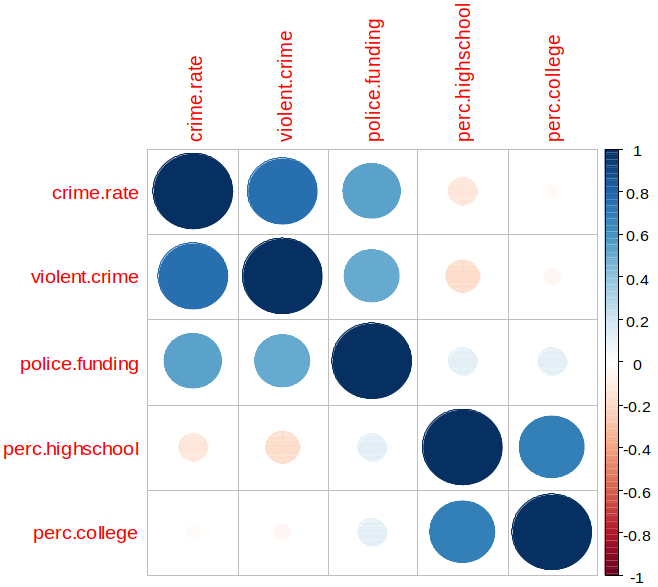
\includegraphics[width = 0.55\textwidth]{PCA/cov_multivariante.png}
\end{center}
Importance of components:
\begin{table}[h]
    \centering
    \begin{tabular}{c|c|c|c|c|c}
         & PC1 &  PC2  & PC3  &  PC4   & PC5 \\
         \hline
         Proportion of Variance & 0.445 & 0.345 & 0.103 & 0.0594 & 0.0479\\ 
         \hline
         Cumulative Proportion & 0.445 & 0.790 & 0.893 & 0.9521 & 1.0000 \\
    \end{tabular}
    \newline
    \vspace{1cm}
    \newline
    \begin{tabular}{c|c|c|c|c|c}
         & PC1 &  PC2  & PC3  &  PC4   & PC5 \\
         \hline
         crime.rate       &	 0.61 &	-0.034  &	 0.31 &	-0.29 &	-0.670 \\
         \hline
         violent.crime    &	 0.60 &	 0.002  &	 0.37& 	 0.02 &	 0.707 \\
         \hline
         police.funding   &	 0.49 &	-0.255 	&	-0.80& 	 0.22 &	-0.009 \\
         \hline
         perc.highschool &	-0.15 &	-0.682 	&	-0.06& 	-0.69 &	 0.177 \\
         \hline
         perc.college    &	-0.07 &	-0.685  &	 0.35& 	 0.62 &	-0.137
    \end{tabular}
\end{table}

\begin{figure}[h]
    \centering
    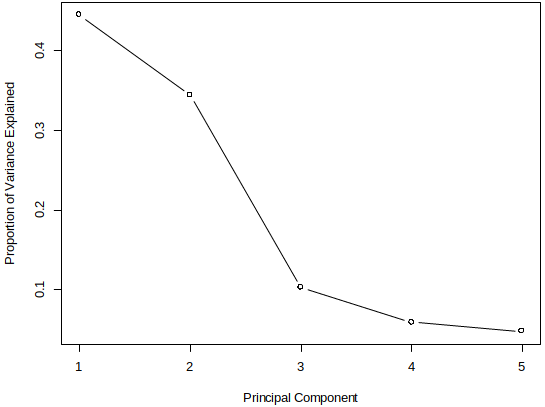
\includegraphics[width = 0.49\textwidth]{PCA/screeplot.png}
    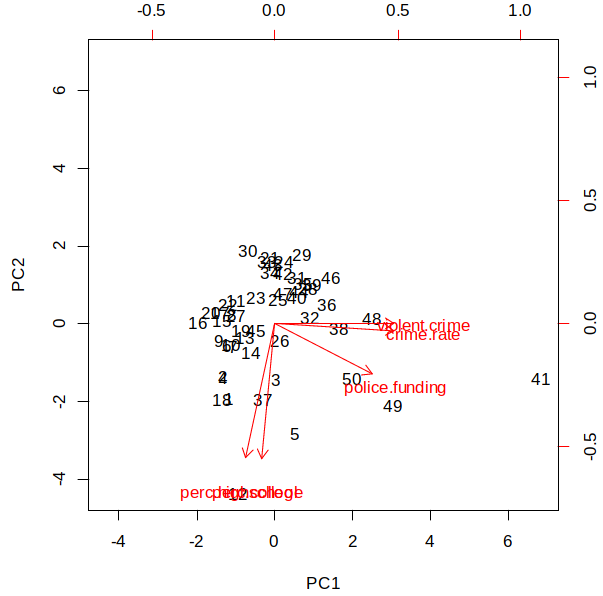
\includegraphics[width = 0.49\textwidth]{PCA/pc1u2plot.png}
    \caption{left side: scree plot. It shows how much of the variation is explained by which PC}
\end{figure}

$\lambda$ is often rescaled and expressed as 'percent of variance explained'. The principal components are extracted such that they explain a maximum amount of variance in the original data. Often a few PCs can capture most of the variance among a large set of original variables. This is true if many of the original variables are correlated:

\subsection{Canonical correlation analysis (CCorA) and Partial least squares regression (PLS)}
Canonical correlation or PLS analyis can be used to study covariation between two sets $X_{1-i}$ and $X_{j-m}$ (are these 10 variables correlated with these 8 variables?).
\begin{itemize}
    \item \textbf{Canonical correlation:} extracts one linear combination of set $X_{1-i}$ and one of $X_{j-m}$, such that this pari of derived variables (=canonical variates) correlates maximally with each other. several orthogonal paris can be extracted
    \item \textbf{Partial least-squares (PLS) analysis:} very simila to canonical correlation, uses covariance matrices and sets of derived variables are not constrained to be orthogonal
\end{itemize}

\begin{lstlisting}
lm(log10(violent.crime) ~ police.funding + perc.highschool + perc.college)

Coefficients:
                 		Estimate 		Std. Error 	t value 	Pr(>|t|)    
(Intercept)      	7.444773   	0.786091   	9.471 	2.23e-12 ***
police.funding   	0.025558   	0.008677   	2.946  	0.00504 ** 
perc.highschool 	-0.053087   	0.016306  	-3.256  	0.00213 ** 
perc.college     	0.054791   	0.031523   	1.738  	0.08888 .  

Residual standard error: 0.8319 on 46 degrees of freedom
Multiple R-squared:  0.2864,    Adjusted R-squared:  0.2399 
F-statistic: 6.155 on 3 and 46 DF,  p-value: 0.001315
\end{lstlisting}
This is a poor model forseveral reasons: There are two crime variables: crime in general (\texttt{crime.rate} and \texttt{violent.crime}) and only one was used. The two educational variables ar highly correlated (using only one would have been better i assume), and the causality is not clearly warranting regression analysis.

\begin{lstlisting}
CCorA(cbind(log10(violent.crime), crime.rate), cbind(police.funding, perc.college, perc.highschool)) 
#X_1-i ~ X_j-m

 Y X
Matrix Ranks 2 3

Pillais trace:  0.47 

Significance of Pillais trace:
from F-distribution:   3e-04 
                       
Canonical Correlations    
CanAxis1 CanAxis2
0.588     0.35
                   Y | X X | Y
RDA R squares      0.328  0.20
adj. RDA R squares 0.284  0.17
\end{lstlisting}

\subsection{MANOVA}
When there are multiple response variables in a design that would ordinarily have been analysed by ANOVA, multivariante ANOVA (MANOVA) (or multivariante analysis of covariance MANCOVA) is used. First, the linear combination Z (a derived variable) is extracted from the matrix of response variables. Z maximizes the ratio of between-group to within-group variance in Z (F-value). This results in a variable that is as 'affected' by the treatment as possible. For one-way MANOVA, this derived variable Z is also called the \textbf{first disciminant function} (because it best 'discriminates' between factor level groups).


\subsubsection{MANOVA on the tadpole dataset}
This allows to statistically test if the food treatment had an effect on tadpole morpholgy, jiontly considering responses in the 7 measured traits. 

\begin{lstlisting}
dat$Pop <- factor(dat$Pop) #Population needs to be a factor 
#just three of the seven traits to illustrate the process:

mod.Man <- manova(cbind(Muscle_depth, Body_depth, Tail_depth) ~ Food, data = dat)
summary(mod.Man)
           Df  Pillai approx F num Df den Df    Pr(>F)    
Food        1 0.65582   187.37      3    295 < 2.2e-16 ***
Residuals 297                                             
\end{lstlisting}

A very high F-value means food seens to have a significant effect (explains a lot of variation)

\textbf{Pillai's trace:} Variance explained by disc. function / (1+variance explained by disc function). \\ 
\textbf{Degrees of freedom for the food effect:} The number of levelsof the factor -1.\\
\textbf{Degrees of freedom for the residuals:} number of observarions - number of effects estimated. \\
Ad for the standerd ANOVA, there is an F-value (var(effect)/var(error)), which, based on the corresponding degrees of freedom, gives the p-value for a combined response to food treatment of all traits considered together.\\
\textbf{right hand side of the MANOVS table:} Denominator DF $\sim$ roughly how many observations you have for the effect. Numberator DF $\sim$ number of estimated means.\par 
More complex models can be fitted with random and nested effects (like the flower pot example). This is shown by including population and considering that populations can respond differently to the food treatment:

\begin{lstlisting}
#first: population as a fixed effect
mod.MAN2 <- manova(cbind(Muscle_depth,Body_depth,Tail_depth) ~ Food*Pop, data=dat )
summary(mod.MAN2)
           Df  Pillai approx F num Df den Df    Pr(>F)    
Food        1 0.70009  218.652      3    281 < 2.2e-16 ***
Pop         7 0.58970    9.891     21    849 < 2.2e-16 ***
Food:Pop    7 0.17703    2.535     21    849 0.0001782 ***
Residuals 283  
#The F-value is even higher here than above probably because the residual variation is smaller (F = individual var./group var.)
#less degrees of freedom because the model is better
#the interaction between food and population is weak (the populations dont react differently to food), but all individuals react strongly (F-Value to food very high)

#second: population as a random effect
mod.MAN3 <- manova(cbind(Muscle_depth,Body_depth,Tail_depth) ~ Food + Error(Pop + Pop:Food), data=dat )
summary(mod.MAN3)
Error: Pop
          Df  Pillai approx F num Df den Df Pr(>F)
Food       1 0.31117  0.60231      3      4 0.6471 #this is weird, but it does not matter
Residuals  6                                      

Error: Pop:Food
          Df  Pillai approx F num Df den Df    Pr(>F)    
Food       1 0.99149   194.25      3      5 1.356e-05 ***
Residuals  7                                             
#approx F-Value still very high because (as seen above) both populations respond about the same

Error: Within
           Df Pillai approx F num Df den Df Pr(>F)
Residuals 283 #the same as in the fixed effect, just DF and error terms are different
\end{lstlisting}

The first model will have more significant results, but will often be less exact.

The F-value and degrees of freedom for the effect of food are calculated by the same principle as for the nested and fixed effect ANOVAs (see lab 2). The F-rations are slightly different for the food effect between model 2 and 3 because the data is unbalanced (not the same number of observations for the two foodtratments in each population). The dataset is balanced enough for the analyses are ok. \par 
What generally can be seen is that it is important o choose the correct random effect. The error terms differ in the number of observations that underlie them, as well as how much variance there is for them. This clearly affects the P-value and comes back to the complicated issue of correctly identifying the true level of replication in the experiment.\par 
The PCs here can be plotted again, this time with the population in different colors:
\begin{lstlisting}
autoplot(tadpole.pca, data = dat, colour = 'Pop',
         loadings = TRUE, loadings.colour = 'blue',
         loadings.label = TRUE, loadings.label.size = 3)
\end{lstlisting}
\begin{center}
    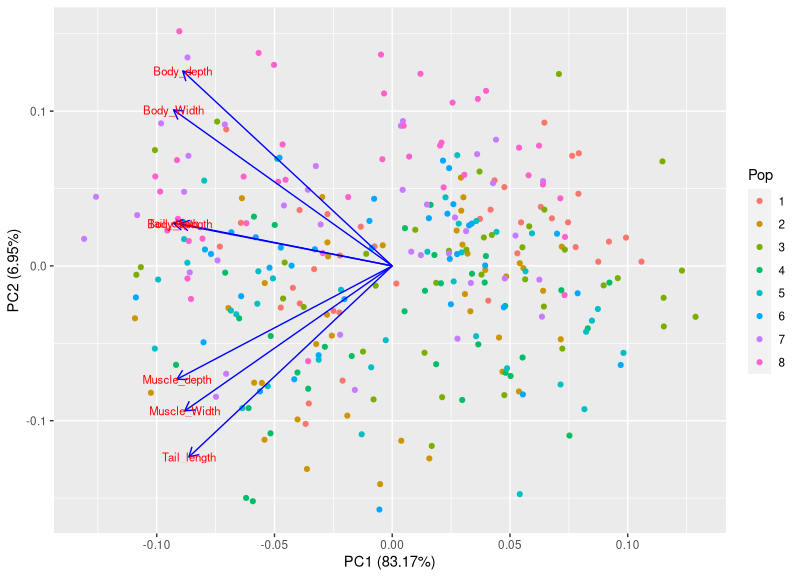
\includegraphics[width = 0.75\textwidth]{lab4/tadpole-pca-food.png}
\end{center}

Population differences should align along PC2, but PC2 explains much less variance in the data compared ot PC1, it remains unclear if these population differences are significant just based on this graph. However, to get at this, the test for population differences could be revisited while also controlling for food effects. In the anova table for model 2 the population effects are significant, but they explain much less variance (lower F-values) compared to the food effect.

\subsection{Linear Discriminant analysis}
This is anaogous to a one-way MANOVA, it is used to classify observations to groups along one dimension (one 'factor') based on linear combinations of variables, and asses the success of such classification. Loadings between original variables and discriminant functions (DF) allow interpretation of which variables contribute most to group differences. Multiple DFs (orhtogonal) can be etracted and ordination of objects in DF space allows visualization of patterns. This is constrained to one-way designs.

\begin{center}
    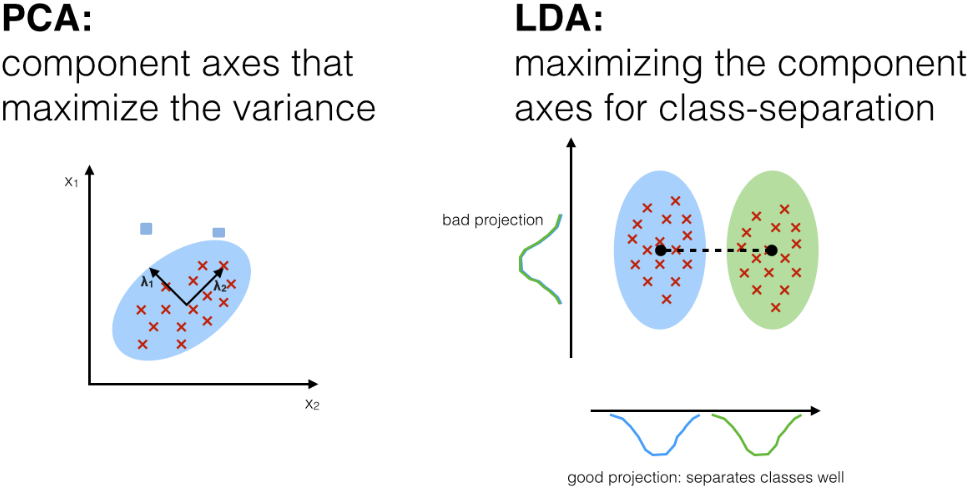
\includegraphics[width = 0.9\textwidth]{PCA/pca-vs-lda.png}
\end{center}


\subsection{Multivariante statistics (lab 4)}
This is a continuation of lab 3, where there were problems because the violent.crime and crime.rate (as independent and dependent variables respectively) were too correlated, and distorted the model outcome. \par 
To solve this problem, multivariante methods can be used where the goal is to reduce data in high dimensional space into something more interpretable (for hypothesis testing).  \\
\textbf{definition from DataCamp:}\\
\begin{small}
\begin{center}
\textit{“PCA is a type of linear transformation on a given data set that has values
for a certain number of variables (coordinates) for a certain amount of
spaces. This linear transformation fits this dataset to a new coordinate
system in such a way that the most significant variance is found on the first
coordinate, and each subsequent coordinate is orthogonal to the last and
has a lesser variance. In this way, you transform a set of x correlated
variables over y samples to a set of p uncorrelated principal components
over the same samples. Where many variables correlate with one another,
they will all contribute strongly to the same principal component.
Each principal component sums up a certain percentage of the total
variation in the dataset. Where your initial variables are strongly
correlated with one another, you will be able to approximate most of the
complexity in your dataset with just a few principal components.”}
\end{center}
\end{small} 
PCA will be shown using the america crime dataset, this time loading it with \texttt{read.table()}. R has a native function for a PCA, called  \texttt{prcomp()}. The weight of the variables relative to each other need to be defined, In this case bott variables are equal. This means that the correlation matrix and not the covariance matrix is used.

\begin{lstlisting}
dat <- read.table('AmericanCrime.txt', header = T)
#extract several data sets and save them as vectors
v.crime <- log10(dat[,2]) #log-transformed again to reduce the influence of the outlier, see lab 3
c.rate <- dat[,1]

PC.crime <- prcomp(cbind(v.crime, c.rate), scale = T)
        #scale = true means that the two variables are weighted equally
summary(PC.crime) 
Importance of components:
                          PC1    PC2
Standard deviation     1.2920 0.5750
Proportion of Variance 0.8347 0.1653
Cumulative Proportion  0.8347 1.0000

PC.Education <- prcomp(dat[,4:5], scale = T)
summary(PC.Education)
Importance of components:
                          PC1    PC2
Standard deviation     1.2966 0.5647
Proportion of Variance 0.8405 0.1595
Cumulative Proportion  0.8405 1.0000
\end{lstlisting}

The output shows how much variance is explained by each principal component (given by their eigen-values) and how they are related to the original variables (given by their eigen-vectors). The first OC explains a great deal of the variation which is why only this is used. For the regression the PC scores for each individual on PC1 are important. They are extracted and used for a regression.

\begin{lstlisting}
pc.crime.scores <- PC.crime$x[,1]
pc.education.scores <- PC.Education$x[,1]
mod <- lm(pc.crime.scores ~ dat$police.funding + pc.education.scores)
summary(mod)
Residuals:
     Min       1Q   Median       3Q      Max 
-2.30491 -0.85342  0.04459  0.64144  2.78439 

Coefficients:
                    Estimate Std. Error t value Pr(>|t|)    
(Intercept)         -1.79070    0.46989  -3.811 0.000402 ***
dat$police.funding   0.04742    0.01171   4.049 0.000191 ***
pc.education.scores  0.21778    0.12484   1.744 0.087618 .  

Residual standard error: 1.123 on 47 degrees of freedom
Multiple R-squared:  0.2755,	Adjusted R-squared:  0.2447 
F-statistic: 8.936 on 2 and 47 DF,  p-value: 0.0005141
\end{lstlisting}

Now, the police funding has a significant of the variance of the crime data again, even though both crime.rate and violent.crime.

\subsubsection{Example 2: iris data}
In the dataset, three species of flowers are measured for four continuous floral traits.

\begin{lstlisting}
data('iris')
levels(iris$Species) #show the different kinds of species in the datasets
#extract measurements by species
iris.setosa <- iris[iris$Species == 'setosa', 1:4]
iris.versicolor <- iris[iris$Species == 'versicolor', 1:4]
iris.virginica <- iris[iris$Species == 'virginica', 1:4]
\end{lstlisting}
The histograms of the different traits can be plotted to see if they are normally distributed (which is a prerequisite to all further analysis) and to see how to potentially transform them. Only petal with deviates (for one species), but it does not improve by log-transformation. Normally, this would require more in-depth research but for simplicity we will leave it as is now.\par 
The PCA can be performed as before usint \texttt{prcomp()}. Scale = True is used again to weigh the variabels evenly.

\begin{lstlisting}
ir.pca <- prcomp(iris[, 1:4] , scale = TRUE)
ir.pca

Standard deviations (1, .., p=4):
[1] 1.7083611 0.9560494 0.3830886 0.1439265

Rotation (n x k) = (4 x 4):
                    PC1         PC2        PC3        PC4
Sepal.Length  0.5210659 -0.37741762  0.7195664  0.2612863
Sepal.Width  -0.2693474 -0.92329566 -0.2443818 -0.1235096
Petal.Length  0.5804131 -0.02449161 -0.1421264 -0.8014492
Petal.Width   0.5648565 -0.06694199 -0.6342727  0.5235971
\end{lstlisting}

The loadings in the eigeh-vectors of each PC represent the correlations between the origina variables and the PC. \par 
Another way to look at loadings are as weights, where the variables contributing more to the PC (i.e. they are more strongly correlated to it) get a higher loading for that PC (but the PC itself might not explain a lot of variance in the data, this is shown by the eigen-value). The sign of the loadings represents the direction of the relationship between each variable and the PC.\par 
How much is the variance explained by each principal component?
\begin{lstlisting}
summary(ir.pca)
Importance of components:
                          PC1    PC2     PC3     PC4
Standard deviation     1.7084 0.9560 0.38309 0.14393
Proportion of Variance 0.7296 0.2285 0.03669 0.00518
Cumulative Proportion  0.7296 0.9581 0.99482 1.00000
\end{lstlisting}

The first principal component explains 0.7296\% of the variance of the entire dataset, the first and second combined then $0.7296+0.2285=0.9581$. The results can also be plotted with the package \texttt{ggfortify}.

\begin{lstlisting}

library(ggfortify)
autoplot(ir.pca, data = iris, colour = 'Species',
         loadings = TRUE, loadings.colour = 'blue',
         loadings.label = TRUE, loadings.label.size = 3)
\end{lstlisting}

\begin{center}
    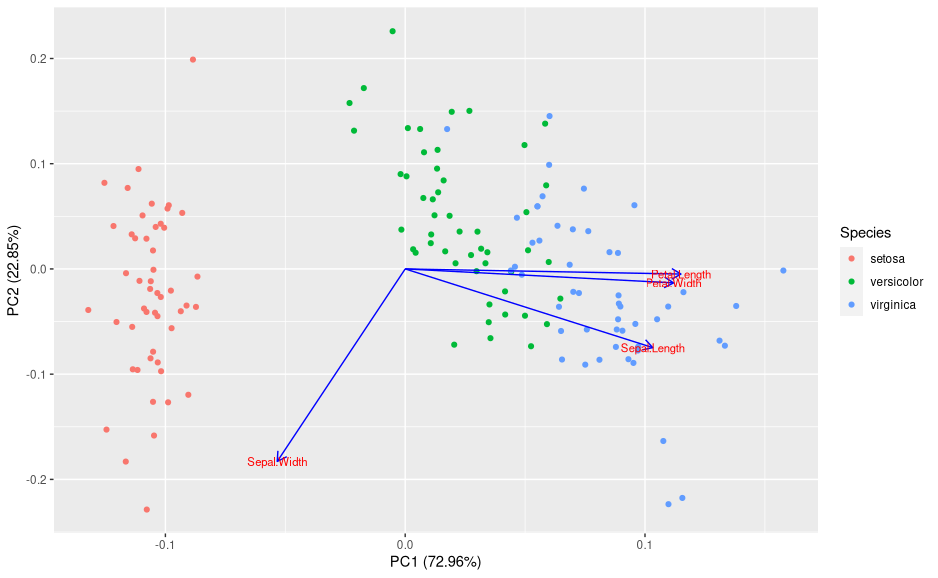
\includegraphics[width = 0.75\textwidth]{lab4/iris-pcs.png}
\end{center}

The direction of the arrows represents the loading on the two PCs for each original variable (compare with \texttt{summary(ir.pca)}. It also tells you something about the differences between the groupings and individual observations, such that points positioned far out in the same direction as an arrow have higher values for the original variable, and points placed far away on the opposite side of the arrow have lower values.\par 
Iris setosa is clearly different. PC2 explains mainly the variation in Sepal size (width and length), but the species are not very different in this aspect. Note also that the arrow vectors along the PC axes correspond directly to the respective trait-loadings on PC1 and PC2 given the summary output from the PCA. The loading for sepal length on PC3 is 0.7195664.

\subsubsection{Example 3: Tadpoles}
The data is 7 morphological traits collected from 8 populations of moor frog tadpoles measured under two treatments (R = restricted and U = unlimited).

\begin{lstlisting}
dat <- read.table('tadpole_food.txt', header = T)
tadpole.pca <- prcomp(dat[,3:9], scale = T)
summary(tadpole.pca)
Importance of components:
                          PC1     PC2     PC3     PC4     PC5    PC6     PC7
Standard deviation     2.4128 0.69766 0.47866 0.42239 0.38967 0.3029 0.20113
Proportion of Variance 0.8317 0.06953 0.03273 0.02549 0.02169 0.0131 0.00578
Cumulative Proportion  0.8317 0.90121 0.93394 0.95942 0.98112 0.9942 1.00000
\end{lstlisting}

To explain at least 96\% of variance in the original data 5 out of 7 principal components are needed. The data can be plotted again with the library \texttt{ggfortify}.



\begin{lstlisting}
autoplot(tadpole.pca, data = dat, colour = 'Food',
         loadings = TRUE, loadings.colour = 'blue',
         loadings.label = TRUE, loadings.label.size = 3)
\end{lstlisting}

\begin{center}
    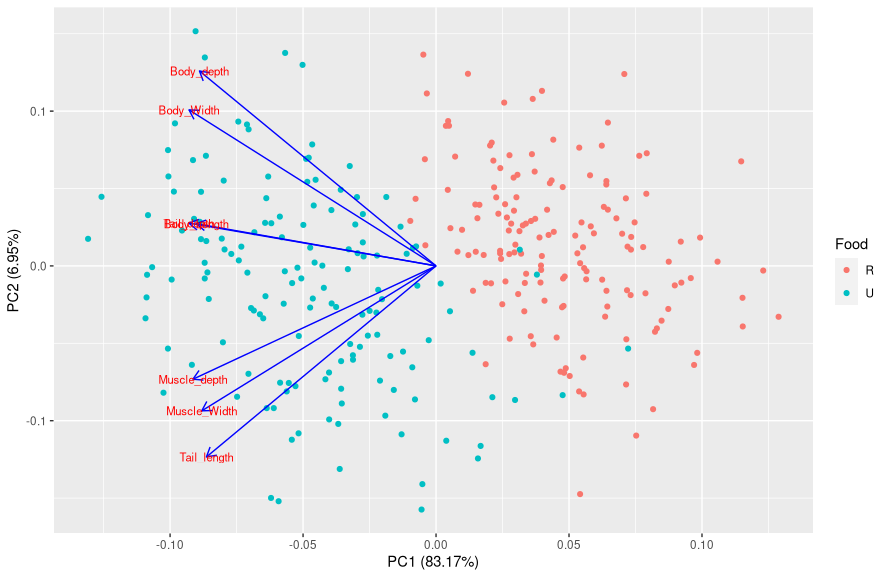
\includegraphics[width = 0.75\textwidth]{lab4/tadpole-pca.png}
\end{center}

From the loadings on PC1 from the summary output we can see that increases in PC1 leads to decreases in all seven traits. The graph above shows that food treatment loads heavily on PC1 and leads to increase in all morphological traits which means that unlimited food leads to increased size. There is much less variation in how body parts grow in relation to each other (PC2 ~ 7\%).\par 
Food treatment does not seem to cause any changes along PC2 (green and red dots only separated in horizontal and not vertical dimension), meaning it did not affect how tadpoles allocate energy to muscle and tail growth relative to overall body size. However, if you instead ordinate populations along PC1 and PC2, then you see that populations seem to differ along PC2 (see MANOVA). 

Uses:
\begin{itemize}
    \item Classification: plcing samples into subsets so that the data in each group shares a common trait (discrete variables)
    \item Ordination: mainly for visualization: serves to sumarize multivariante data by producing low-dimensional ordination space with similar spaces plotted close together (continuous) (is also possible without guidance from explanatory variables (indirect)).
\end{itemize}

\subsubsection{relationship between ordination and regression}
\renewcommand{\arraystretch}{1.5}
\begin{table}[h]
    \centering
    \begin{tabular}{c|c|c}
         \textbf{Data to explain} & \textbf{Explanatory varables} & \textbf{Analysis} \\
         \hline 
         1 variable & 1 variable & simple regression \\
         \hline
         1 variable & m variables & multiple regression \\
         \hline
         p variables & / & simple ordination \\
         \hline 
         p variables & m variables & canonical ordination 
    \end{tabular}
\end{table}
\renewcommand{\arraystretch}{1}

Simple ordination - indirect gradient analysis: \textbf{PCA}, Principal Coordinates analysis (PCoA), non-metric multidimensional scaling (NMDS)\\
Canonical ordination - direct gradient analysis: Canonical correspondance and correlation analysis (CCA and CCorA), Redundancy analysis.\par 
Anova does not fit in here, because there are already predefined groups in ANOVA (are the groups significantly different?), this is used to divide the data into groups. If there is an effect that devides the groups, these methods will find them anyway. 

\subsubsection{Dissimilarity/similarity}
There is always the common denominator, there is alwas a measure of difference or similarity between the variables (simple for one variable, increasingly different for more observations). The simples most often used measure is euklidian distance (put all variables in a high dimensional coordination system and calculate their distances). \par 
This is impossible to visualize for dimensions higher than three, which is why you can make a similarity/dissimilarity distance matrix that shows how far away each sample is fom each other sample based on their values for each measured variable (coordinates).\par 
Highly expressed genes will dominate this analysis, which means the per gene expression needs to be standardized (divide all values by the max. value or variance standardize so that all have the same mean expresison). The mean level of gene expression often differs among samples/libraries, which is why the libraries need to be normalized to be actually compareable (there are R packages for that, can be done in the same way as the variables).\par 
When both libraries and genes (variables) are standardized, the result is the correlation matrix. Everything from here on can be done on 'raw' and standardized data, even though results and interpretation will differ.\par 
Samples can be classified and sorted into groups as already discussed, but this is also possible for genes ('these genes show the same pattern of expression across samples'). This is not possible for every technique.\par 
The goal is to cluster the data (classification), this means to group samples so thst the data in each cluster share some similarity, those methods are based on similarity matrices. The common major classes are hierarchical and non-hierarchichal clustering.

\textbf{K-means (non hierarchical) clustering}: K-means clustering aims to assign objects to a user-defined number of clusters (k) in such a way that maximizes the separation of those clusters while minimizing intra-cluster distances relative to the cluster's mean or centroid. The algorithm typically defaults to Euclidean distances, however, alternate dissimilarity measures can be accepted by many implementations. The user is usually expected to set 3 parameters: 1) the number of clusters expected (k), 2) the initialization method (analysis needs to start somewhere), and 3) the distance metric (e.g. eiclidic) to be used.\par 
The challenge is to find out which number of clusters fits the data best.

\textbf{hierarchichal clustering}: Uses a dissimilarity matrix to produce dendrograms (trees) with hierarchical clusters that are built ”bottom-up”. Several different options and different measures of dissimilarity can be used, the ranch lengths are informative. This is common in many areas of biology. Statistical support for nodes can be provided by resampling, meaning the experiment can be repeated to see if the tree shows up again (possibly by reshuffling the data.\par 
One method is complete linkage clustering. The two samples with the smallest distance in the similarity matrix are selected and merged into a new sample. The distances to the other samples from this new merged sample is the max distance it had to one of the merged samples (distance to merged1: 3, distance to merged2: 5 $\rightarrow$ distance to merged 2 is selected as new distance to the merged point).

\subsubsection{Ordination}
The typical aim is to reduce multivariante data (for example, many genes) into fewer dimensions used to seperate samples. These can then be used to plot samples (typically in 2D [=bivariate] space) in order to visualize and seek patterns. Similar samples are close together in such bi-plots, and dissimilar samples are placed far apart. \par
A very large number of different methods available – only the common ones are mentioned here.
This works as follows:\par 
New derived variables (Z$_{ij}$), that we call principal components or axes or dimensions, are created. Methods differ in how these derived variables are attained, but all are constructed from our data, based on either a dissimilarity matrix or the variance-covariance matrix.\par
\textbf{Principal component analysis}: On the continuous raw data using euklidian distance. Applied to covariance- or correlation matrix based on original data, the Dimensions/axes called ”principal components”. Axes capture maximal variation in the original data and are orthogonal to each other.
It is a good starting point to find trends in the data when p>n and can then be used for further analysis.\par
\textbf{Principal Coordination analysis}: (aka metric multidimensional scaling) More flexible than PCA, can be non-euklidian and non-continuous in creating the similarity matrix, then PCA on that matrix. It maximizes the correlation between dissimilarity matrix and ordination distance $\rightarrow$ ordinates samples along the multivariate dimension(s) that best separate objects. If the dissimilarity matrix is based on Euclidean distance in the original data, eigen-analysis on dissimilarity matrix will generate the same result as a PCA on the original data. It is difficult to get an intuitive feeling how the scores along the PCoA axis to the original data because they are further removed from it.\par
\textbf{non-metric multidimensional scaling (NMDS)}: similar to PCoA but uses ranked data (1, 2, 3, 100 $\rightarrow$ 1, 2, 3, 4) and is more robust for this reason. It also uses the similarity matrix, the dimenstions are called coordinates or axes. The number of axes needs to be predetermined. It returns 'Stress' (how well the analysis fits the data): $>$0.2 poor, $<$0.05 excellent. The stress decreases when there are more ordination dimensions allowed.\par

All of these Methods are indirect, which means they are naive to underlying casual variables and the grouping/gradients are only based on gene composition/expression data. Directo ordination methods seek covariation between response data and causal explanatory variables.

\subsubsection{direct gradient analysis}
The response variables should guide how the PCs are created, not just compared after as in PCA. ”Simple” linear regression between derived variables (dimensions/axes) and e.g. environmental variables can be used, but the power is typically quite low. Better but more complex multivariate methods: Redundancy analysis (RDA, lab 5), Canonical correspondence analysis(CCA), Canonical correlation analysis (CCorA) .\par
Standardization is very important.
\textcolor{red}{slide 23, 24 multivariante analysis 2}\par 

\begin{figure}[h]
    \centering
    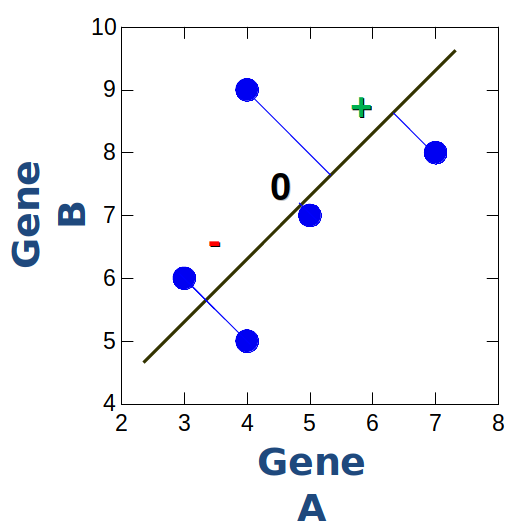
\includegraphics[width = 0.49\textwidth]{PCA/1PC.png}
    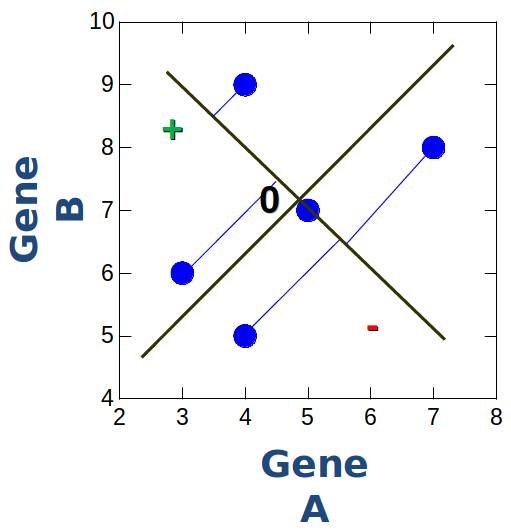
\includegraphics[width = 0.46\textwidth]{PCA/2PC.png}
\end{figure}

\begin{table}[h]
    \centering
    \begin{tabular}{c|c|c|c|c}
         sample & A & B & PC1 & PC2 \\
         \hline 
         1 & 3 & 6 & -2.1 & 0.4 \\
         \hline
         2 & 5 & 7 & 0.1 & 0  \\
         \hline
         3 & 4 & 5 & -2.1 & -0.7 \\
         \hline
         4 & 7 & 8 & 1.9 & -0.8 \\
         \hline
         5 & 4 & 9 & 0.6 & 1.9 \\
    \end{tabular}
    \caption{See figure below for visualization}
\end{table}
Axes are created how the envireonmental variables affect the species composition, shows how envireonmental variables cause sectioning. Ways to test whether the results are significant (see lab 5)\par 

\newpage 
\textbf{RDA - redundancy analysis}
Reduces dimensions via PCA on the set of response variables (y), conditinoed on their covariation with the set of explanatory variables (x)
\begin{enumerate}
    \item Multiple regression (MLR) $$\sum_{1-p} (y_i | x_{1-m}) \rightarrow \hat{y}_{1-p}$$
    \item PCA $\rightarrow \: \hat{y}_{1-p}$
\end{enumerate}
Significance tests of assiciations between ordination axes and explanatory variables by permuation can also be conducted. PCA can also be applied on the residual (unconstrained) variance.\\
\textbf{summary of common ordination techniques}
\begin{itemize}
    \item Indirect gradient analysis
    \begin{itemize}
        \item Distance-based approaches: \\
			Principal Coordinates Analysis - PCoA (Metric multidimensional scaling) \\
			Nonmetric Multidimensional Scaling, NMDS
		\item Eigen analysis based approaches\\
			Linear model: Principal Components Analysis, PCA \\
			Unimodal model: Correspondence Analysis, CA
    \end{itemize}
    \item direct gradient analysis
    \begin{itemize}
        \item Linear model\\
			Linear regression (of principal components) \\
			Canonical correlation analysis, CCorA \\
			Redundancy Analysis, RDA
		\item Unimodal model \\
			Canonical Correspondence Analysis, CCA
    \end{itemize}
\end{itemize}


\textbf{some final notes:}
\begin{itemize}
    \item \textbf{  It is not always clear when to use which method!}
    \item Cluster analysis and ordination are useful tools for description and visualization.
    \item Scaling/Standardization of response data can affect interpretation
    \item For direct gradient analysis, the number of explanatory variables must be smaller number of samples (n)
    \item As in any regression model, carefully consider scaling of explanatory variables a priori, based on their presumed relationship with genomic response data
    \item Ordination is ypically used for exploratory data analysis - usually not meant for hypothesis testing! (some null hypotheses can be tested with appropriate resampling tests in direct ordinations)
\end{itemize}


\subsubsection{ordination: k means clustering (lab 5)}
K-means clustering can be used to determine how many clusters the data likely consists of, it can be run on raw continuous, or distance based data. The clustering algorithm works by ordering data points into k number of clusters by finding groups such that the variance in the distance to the center of each cluster and the respective data is minimized. There are several R-packages needed for the following analysis:
\begin{lstlisting}
pkgs <- c("factoextra", "NbClust", "cluster", "fpc", "gridExtra", 'car', 'ggplot2' ...)
install.packages(pkgs)
library(factoextra)
library(NbClust)
library(cluster)
library(fpc)
library(gridExtra)
library(ggfortify)
library(vegan)
library(psych)
library(ggplot2)
\end{lstlisting}
The tadpole data set from before is used again here. non-hierarchical k-means clustering is performed.

\begin{lstlisting}
setwd('~/MEGAsync/Bioinformatik MSc/Semester 1/intro to programming/statistics/lab5/')
tadpole <- read.table("tadpole_food.txt", header=TRUE)
dat <- scale(tadpole[3:9])
#cluster the data into 2, 3, 4, 5 clusters respectively
k2 <- kmeans(dat, centers = 2, nstart = 25)
k3 <- kmeans(dat, centers = 3, nstart = 25)
k4 <- kmeans(dat, centers = 4, nstart = 25)
k5 <- kmeans(dat, centers = 5, nstart = 25)
#plot the results
p1 <- fviz_cluster(k2, genom = 'point', data = dat) + ggtitle('k=2')
p2 <- fviz_cluster(k3, genom = 'point', data = dat) + ggtitle('k=3')
p3 <- fviz_cluster(k4, genom = 'point', data = dat) + ggtitle('k=4')
p4 <- fviz_cluster(k5, genom = 'point', data = dat) + ggtitle('k=5')
grid.arrange(p1, p2, p3, p4, nrow = 2)
\end{lstlisting}

\begin{center}
    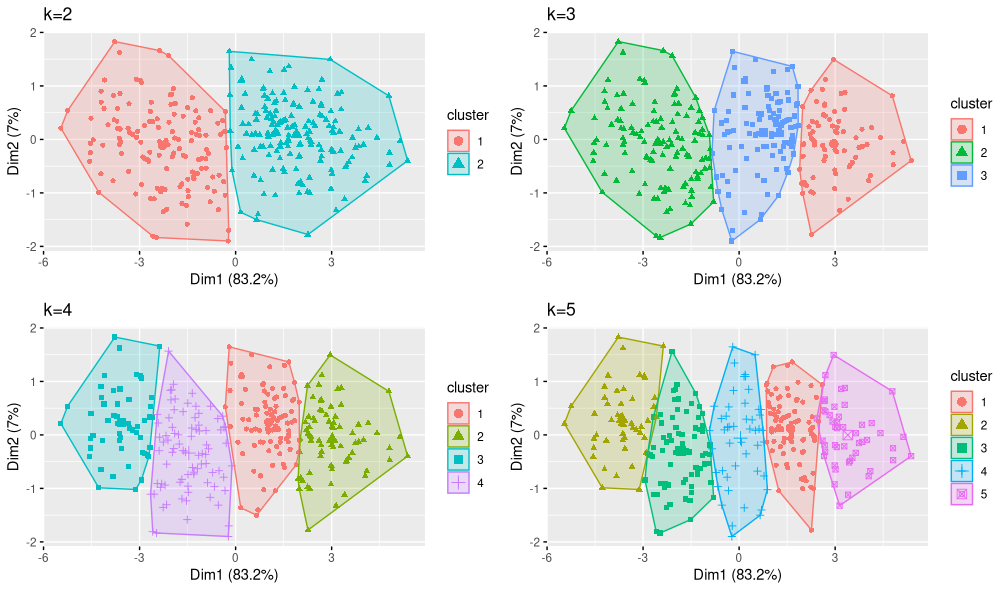
\includegraphics[width = 0.99\textwidth]{lab5/kmeans.png}
\end{center}

It can be judged which amount of clusters is best as follows:

\begin{lstlisting}
fviz_nbclust(dat, kmeans, method = "silhouette") + labs(subtitle ="Silhouette method")
\end{lstlisting}

\begin{center}
    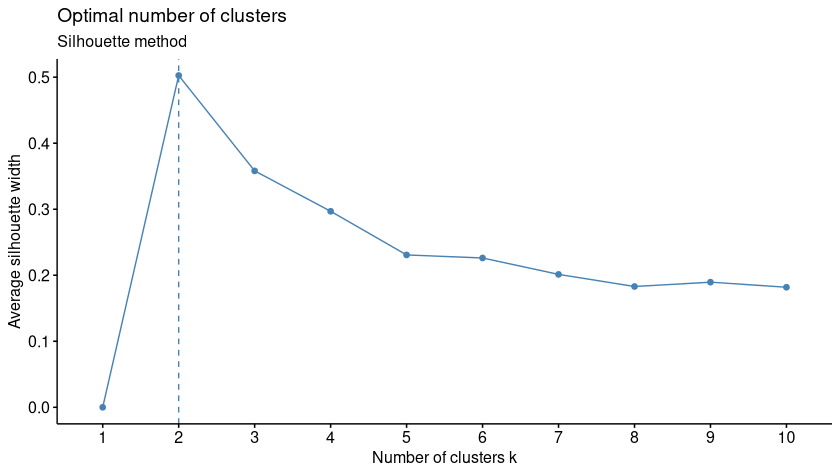
\includegraphics[width = 0.9\textwidth]{lab5/kmeans_ranking.png}
\end{center}

k = 2 is obviously the optimal number of clusters. This makes biological sense, because there are two treatments (unlimited and restricted food) that influence the measurements.

\subsubsection{ordination: hierarchical clustering (lab5)}
In hierarchical clustering the number of clusters does not need a predefined number of clusters. Clustering is presented as a tree-like structure.

\begin{lstlisting}
d <- dist(dat, method = 'euclidian')
hc1 <- hclust(d, method = 'complete')
par(mfrow=c(2,2))
plot(hc1, cex = 0.6, hang = -1)
rect.hclust(hc1, k = 2, border = 2:5)
plot(hc1, cex = 0.6, hang = -1)
rect.hclust(hc1, k = 3, border = 2:5)
plot(hc1, cex = 0.6, hang = -1)
rect.hclust(hc1, k = 4, border = 2:5)
plot(hc1, cex = 0.6, hang = -1)
rect.hclust(hc1, k = 5, border = 2:5)
par(mfrow=c(1,1)) 
\end{lstlisting}

\begin{center}
    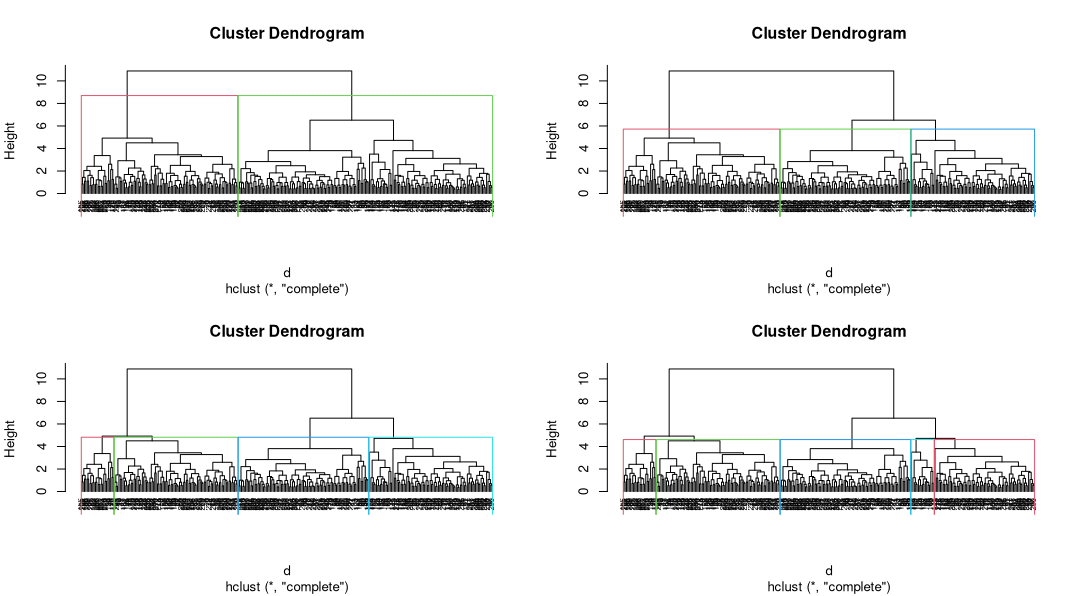
\includegraphics[width = 1.12\textwidth]{lab5/hierarchical.png}
\end{center}
Here, it seems again like 2 clusters make the most sense (branch lengths are important). Hierarchical subclustering (that might be biologically important) may also be seen in this method

\subsubsection{PCoA (aka classical multidimensional scaling, mds) in R}
The method works on distance matrices and after dimensionality reduction, it plots data points depending on dissimilarity and their respective association to the coordinate axes. In classical PCA, the dimensions of the dataset are to be reduced while keeping as much information (variance) as possible, while here, the distance matrix is the starting points and the goal is to find how the distance between the points and their location are situated in reduced dimensional space. \par 
The key is the choice of distance measure, but it is highly dataset specific and it can impact the analysis in a negative way

\section{Problems with previous methods}

Alternatives to the frequentist approach (what we did so far with the null hypothesis, more flexible than anova (that presumes the null hypothesis).

\textbf{problems with frequentist methods}
\begin{itemize}
    \item Data often do not conform to the assumptions of “standard statistical tests”. Resampling statistics is a practice that allows a flexible way to test most hypotheses without constraining assumptions.
    \item Sometimes “null hypotheses” are weird to think about for some hypotheses. Like modelling sequence data for which there are very strong priors (a priori predictions) for how these sequences can change (that might want to be included into the predicted framework).
    \item We ideally want to incorporate prior knowledge into the analysis, weighting the likelihood of different outcomes by this prior knowledge. For this we can use Bayesian statistics.
    \item Analytical solutions to these sometimes very complex models is almost impossible. We can then use simulations to find the most probable result given our data. Markov Chain Monte Carlo simulations is one popular and “economic” (relatively speaking) method to do this.
\end{itemize}

\textbf{problems with multivariante methods}
\begin{itemize}
    \item Constrained ordination methods such as CCA and RDA find the 'best possible' relationship between response and explanatory variables. Therefore, we can observe strong relationships, even with randomized data. We are interested in whether our ordination is 'stronger', than expected due to chance. (This is not a random process, but how good are the results/PCs)
    \item In eigenanalysis-based methods (e.g. PCA, CA, CCA, RDA), the eigenvalue is a reasonable measure of the strength/explanatory power of an ordination axis. But these numbers also follow statistical distributions (e.g. Chi-squared). So classical statistical testing is problematic.
\end{itemize}

Example:

\begin{center}
    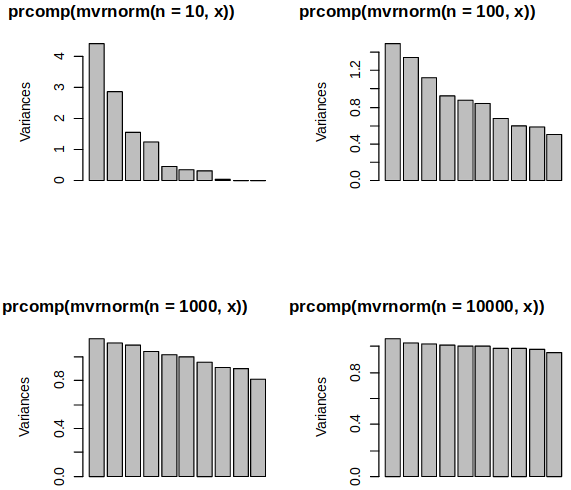
\includegraphics[width = 0.75\textwidth]{bayesian/pca_res.png}
\end{center}
PCs of datasets, for only 10 samples PC1 explains the most variance by chance. but for more individuals all PCs describe the same amount of variation. This has less sampling error and is closest to reality. Is there a possiblity

For top left: if the code is run often and every time PC1 is extracted, then its mean can be calculated. if the PC1 from another dataset is 95\% bigger/smaller than this mean PC from a random dataset, there might be a non-random signal in the data.

\section{Resampling}

\subsection{Randomization and permutation test}

\begin{itemize}
    \item Require no particular assumptions concerning statistical distributions. 
    \item Focused on providing a robust P-value
    \item Permutation  and randomization tests are increasingly applied even in the context of traditional statistical tests (e.g. correlation, t-tests, ANOVAS, etc.).
    \item Computationally demanding and need to be specifically defined for each experiment. Does not provide parameter estimates and confidence limits.
\end{itemize}

Procedure for a randomization test:

\begin{enumerate}
    \item Devise a test statistic which is large if your observed effect is strong
    \item Define your null hypothesis.
    \item Create a new data set consisting of your data, randomly rearranged. 
    \item Calculate your test statistic for this data set, and compare it to your true value. 
    \item Repeat steps 3 and 4 many times (preferably several hundred).
\end{enumerate}

The general idea is that the statistical significance of an association (or something else) can be evaluated by comparing the observed associaction with a distribution of associations obtained by randomly reordering the datapoints. If the true test statistic is greater than 95\% of the random values, then you can reject the null hypothesis at p<0.05. (one tailed vs. two tailed test - if the latter, you will need to use a 97.5\% cutoff). 

\subsubsection{Yanomama villages example}
There is a dataset wirht the genetic and geographic distances computed for 19 villages of the Yanomama Amerindians. The data is to be tested for a relationshp between geographic and genetic distances. There is a distance matrix for both that contains the distance from every village to every other village. These Data points can be plotted (genetic distance on y and respective geographic distance on x). There is a slight upwards trend to be observed, but is it significant?\par 
There are 171 data points, but for only 19 truly independent villages $\Rightarrow$ randomization test! It would be some kind of pseudo-replication to use all 171 data points as if they are independent. (randomize the numbers in the matrix to compare to the original matrix, pairwise distances between the villages, just 'nested' or 'random' effect not enough.)


\subsubsection{Mantel test of association}
The best way to test for association between geographic and genetic distances, it can be applied when there are two matrices or distances or dissimilarities between units. In a Mantel test program, the correlation r between the elements of the two matrices is first computed. Next, there is a random reordering of the units for one of the matrices and the correlation between this matrix and the other one is computed. This is repeated many times and the proportion of times the correlation is stronger than for the observed cas is noted. This proportion is the simulated p-value. \par 
For the Yanomama village data the observed correlation is r = 0.510. The \texttt{mantel.randtest()} function from the \texttt{ade4} package can be used to determine a (one tailed) p-value with 10000 replicated random reorderings: the p-value is 0.0001. The distribution of the 10000 correlations from the Mantel randomization test can be plotted in a histogram, see figure \ref{yanomama}.

\begin{figure}[h]
    \centering
    \label{yanomama}
    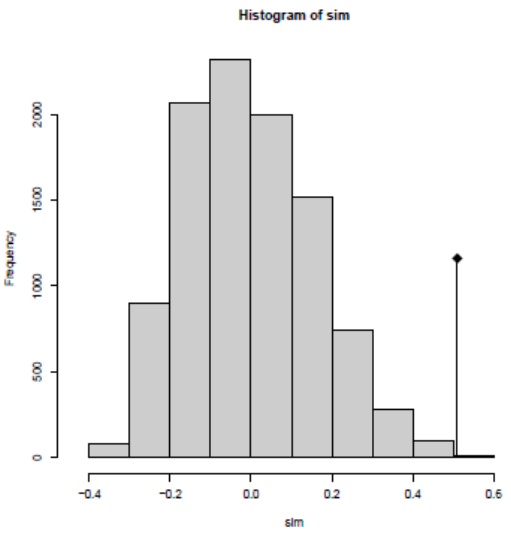
\includegraphics[width = 0.5\textwidth]{bayesian/Mantel-corr-hist.png}
    \caption{The observed correlation of the yanomama dataset is indicated, the simulated p-value is the proportion to the right of this point.}
\end{figure}


\subsubsection{Bootstrap}

\begin{itemize}
    \item The bootstrap procedure is to take N computer generated samples from the observed data (N = 10000 is a resaonable value). Sampling is dome using computer generated random numbers. Each computer generated samples has size n (original size) and is performed with replacement.
    \item This means that there will be typically be duplicates and 'missing' values in a vćomputer generated sample
    \item For each computer generated sample, the value of a statistic (like the mean or the skewness) is computed and stored
    \item This bootstrapped distribution is used to find things like a bias and confidence intervals
    \item in the R package \texttt{boot} functions \texttt{boot()} and \texttt{boot.ci()} can be used for bootstrapping (but they are difficult to figure out)
    \item A great advantage of bootstrap is that very few assumptions about the shapes of distributions are needed
\end{itemize}

\section{Bayesian statistics}
Is traditionally seen as a fringe activity, but now becoming more mainstream. Basic Idea: \\
unknown parameters in models have a probability distribution (\textbf{prior} distribution). The data updates the knowledge to a \textbf{posterior} distribution, this happens using '\textit{Bayes rule}'. It agrees with traditional conclusions in simple cases and is easy to extend to complex models. It is also now supported by efficient computational (simulation) approaces like Markov chain monte carlo (MCMC). Social conventions  in the scientific community on how to make use of it are developing. 

\subsection{Bayesian interference}
\textbf{frequentists inference:} Expresses the probability of observing data, given a particular parameter value (the null hypothesis). Data are repeatable, parameters are not ($P(data|parameters)$)\\
\textbf{Bayesian inference:} expresses the probability of a particular parameter value, given data. The parameters are uncertain, the observed data are not $P(parameters|data)$. This means that prior beliefs are defined which are then exposed to data and then updated into modified posterior beliefs.\\

\subsection{Bayes Theorem: technical}
The probability of the parameters A given the data B: $$P(A|B) = \frac{P(B|A) P(A)}{P(B)}$$ 

\begin{itemize}
    \item $P(B|A)$ is the posterior probability
    \item $P(A|B)$ is the posterior probability of A
    \item $P(A)$ is the prior probability of A
    \item $P(B)$ is the prior distribution
    \item $A$ is the parameters of the model
    \item $B$ is the observation/data
\end{itemize}

\subsection{Is he a zombie?}
If someone was tested positive for a zombie virus and the test has 99\% accuracy, what is the probability that he is actually a zombie? That depends on the amount of zombies in the general (tested) population. If a test is positive in a population with 1\% zombies (and every one else tested negative) the probability of not being a zombie despite a positive test.

\renewcommand{\arraystretch}{1.5}
\begin{table}[h]
    \centering
    \caption{zombie population: 50\% (left) and 0.5\% (right)}
    \begin{tabular}{c|c|c|c}
         & positive test & negative test & total \\
         \hline 
         infected & 9900 & 100 & 10000\\ 
         \hline 
         Healthy & 100 & 9900 & 10000 \\
         \hline 
         total & 10000 & 10000 & 20000
    \end{tabular}
    \begin{tabular}{c c}
           &    \\
           &  
    \end{tabular}
    \begin{tabular}{c|c|c|c}
         & positive test & negative test & total \\
         \hline 
         infected & 99 & 1 & 100\\ 
         \hline 
         Healthy & 199 & 19701 & 19900 \\
         \hline 
         total & 298 & 19702 & 20000
    \end{tabular}
\end{table}
\renewcommand{\arraystretch}{1}
From Those tables, the true positives can be calculated, meaning the amount of people that had a positive test and were infected. The prior Hypothesis is the prevalence of zombies in the population. Abbreviations: inf = infected, + or - = positive or negative test.
\begin{equation*}
    P(inf|+) = \frac{P(inf) \cdot P(+|inf)}{P(+)}
\end{equation*}
calculate with the above table:
\begin{equation*}
\begin{split}
    50 \% \; zombies\;\;\;\;\;\;\;\;\;\;\;\;\;\;\;\;\;\;\;\;\;\;\;\;\;\;\;\;\;\;\;\;\;\;\;\;\;\;\;\;  &  0.5\% \; zombies \\
    \frac{0.5 \cdot 0.99}{0.5 \cdot 0.99 + 0.5 \cdot 0.01} = 0.99 \;\;\;\;\;\;\;\;\;\;\;\;\;\;\;\; & \frac{0.005 \cdot 0.99}{0.005 \cdot 0.99 + 0.995 \cdot 0.01} = 0.33
\end{split}
\end{equation*}

\subsection{importance of the correct priors}
Wrong priors can lead to drastically wrong assumptions. the result of the probability of being actually a zombie with a positive test in the example above depends greatly on the prior assumption, how many infected people are there in the population. If this estimate is wrong, the result would be very unreliable.
\begin{center}
    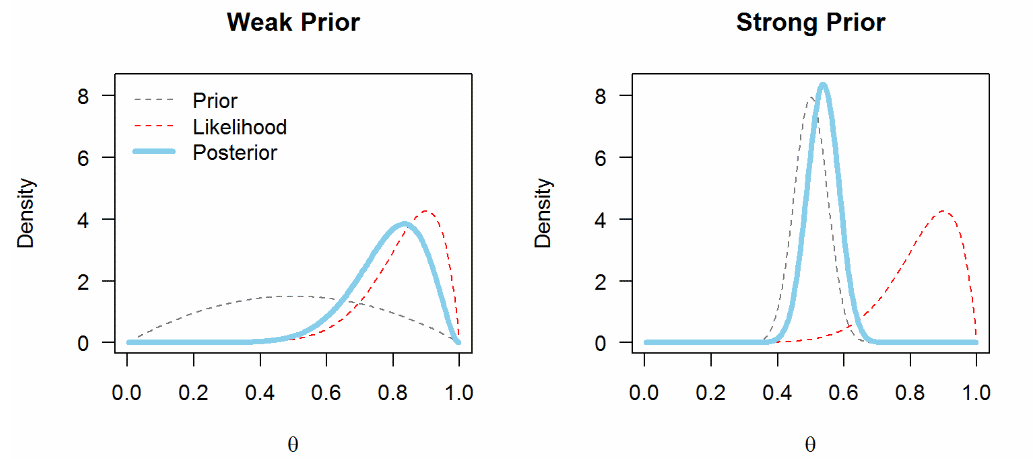
\includegraphics[width = 0.9\textwidth]{bayesian/priors-bayesian.png}
\end{center}
A weak prior is a very general assumption, a string prior is very specific.

\subsection{Pros and cons of bayesian statistics}
\begin{minipage}{0.45\textwidth}
\textbf{PRO}
\begin{itemize}
    \item offers a framework to deal with all the uncertainty. Expresses beliefs beyond Type I and Type II errors
    \item makes use of more information, not just the data in the particular experiment
    \item The bayesian paradigm is very flexible and intuitive, it can tackle problems that frequentist techniques can not.
\end{itemize}
\end{minipage}
\begin{minipage}{0.45\textwidth}
\textbf{CON}
\begin{itemize}
    \item often considerably more complex than frequentist methods
    \item limitations on hypothesis testing, somewhat inclear inferences
    \item limited software to give 'off-the-shelf' analyses
    \item Subjectivity: all the inferences are based on somebodys beliefd, priors are a major problem.
\end{itemize}
\end{minipage} 

\subsection{Markov chain Monte carlo modelling (MCMC)}
A strategy to fit models based upon Bayesian inferences whith has gained some ground as of lately.\\
\textbf{Markov Chain:} a random process that undergoes transitions from one state to another on a state space. It is "memoryless": the probability distribution of the next state depends only on the current state and not on the sequence of events that preceded it. Taking a “step” or not depends on changes in the likelihood of observing data.\\
\textbf{Monte Carlo:} a class of algorithms that rely on repeated random sampling to compute their results, such as generating probability distributions. In MCMC, these algorithms are started (“fed”) with specific prior probability distributions – one for each parameter being estimatated.\\

MCMC goes 'uphill' in the parameter space, guided by the likelyhood of observing data given a MC model (like finding the maximum of a function).
\begin{center}
    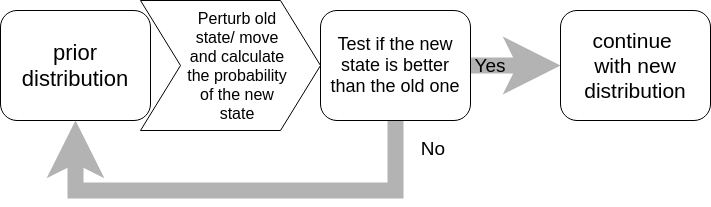
\includegraphics[width = 1\textwidth]{bayesian/MCMC-flowchart.png}
\end{center}
The workflow is repeated for x number of simulations.\par 
What if there are multiple 'optimal' states?
\begin{center}
    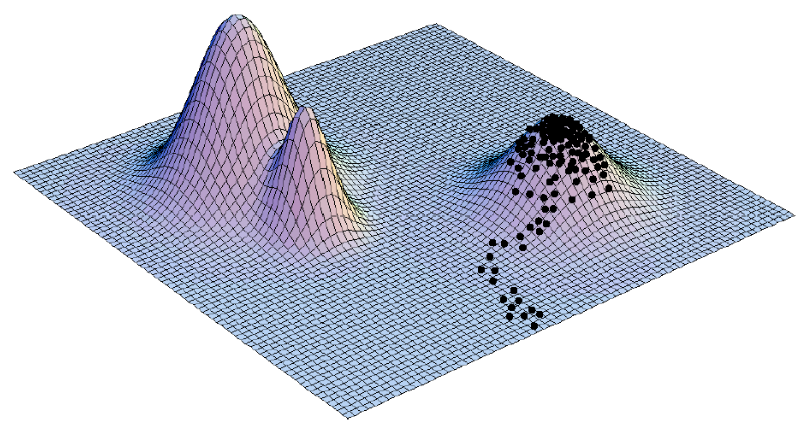
\includegraphics[width = 0.49\textwidth]{bayesian/MCMC-graphic.png}
    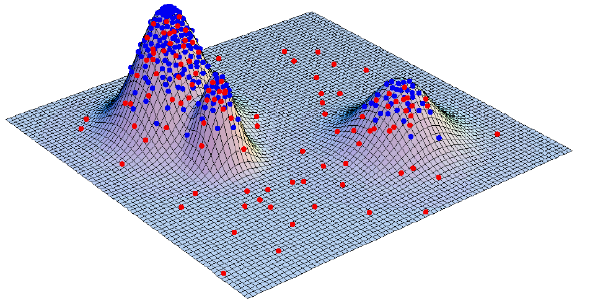
\includegraphics[width = 0.49\textwidth]{bayesian/MCMC-figure-2.png}
\end{center}
The Method gradually chooses the next better model and may therefore only find a local maximum, not an absolute one. This can be solved by running many chains with different initial conditions. MC walks can also use different logics for generating the new state, heated chains, that use a more permissive 'move' criterion. \par 
Metropolis-coupled markov chain monte carlo modelling (MCMCMC) runs parallel chains of which n-1 are heated - exchange information between chains and use cold chain for inference.

\subsubsection{MCMC pros and cons}
\begin{minipage}{0.45\textwidth}
\textbf{PRO}
\begin{itemize}
    \item very flexible
    \item allows fitting models and estimating relatively many parameters with few observations (high parameter/data ratio)
    \item Makes statements about beliefs (95\% Cl:s) and avoids the inferential problems that frequentists face (although modern methods still implement significance testing)
    \item Provides an almost 'non-parametric' analysis, few assumptions about the shape of the posterior distribution
    \item relatively easy (sometimes) to do: extant software
\end{itemize}
\end{minipage}
\begin{minipage}{0.45\textwidth}
\textbf{CON}
\begin{itemize}
    \item 'Models' are very complex, involve choices which greatly affect the outcome
    \item disruption of states only estimates the true posteriors if the Markov chain is 'appropriately' constructed, which is often unclear
    \item \textbf{Subjectivity:} if well-informed priors are not at hand (usually), the path is unclear. Various solutions to this problem: 'weakly informative priors (WIPs)', 'least informative priors (LIPs)', 'flat priors' (not shown to be improper), etc. However, there are no truly uninformative priors.
\end{itemize}
\end{minipage} 
 \par 
\vspace{0.5cm}
It is a controversial field, many diverging opinions.

\section{good statistical practice}
\begin{itemize}
    \item \textbf{Be clear and transparent about your data!} Give sample sizes, all factors, details on sampling methods, etc.
    \item \textbf{Make data publically available!} e.g. journal homepage, NCBIm dryad, etc.
    \item \textbf{Give estimated parameters!} SE:s or CI:s and effect sizes, not only p-values.
    \item \textbf{Be clear and transparent about the analyses:}
    \begin{itemize}
        \item \textbf{avoid p-hacking:} if multiple models are run, then clearly state so and define which ones you choose to rely upon and why.
        \item \textbf{avoid HARK (Hypothesizing After the results are known):} be clear and transparent about expectations and a priori predictions, if results are surprising then say so.
        \item \textbf{avoid selective reporting/reporting bias:} make full use of online appendicies for all analyses made and put them in the main article if possible.
    \end{itemize}
\end{itemize}
Ethical rule-of-thumb: be clear and transparent about your methods, data and the analyses! We all make smaller or larger mistakes – the important thing is that the reader is given full opportunity to assess your data and statistical analyses.

\section{Experimental design in Biostatistics (Mareike)}

How to partition variation of an interesting biological signam from envireonmental noise and confounding factors

\begin{itemize}
\item define a testable hypothesis
\item understand variation in \textit{your} system and how to control it
\item know how the data will be analysed
\end{itemize}

\textbf{sampling goals}
\begin{itemize}
\item minimize systematic errors
\item minimize unwanted variability
\item generalize to a wider population
\end{itemize}

\subsection{types of studies}

\subsubsection{observational, mensurative}
can find association which can best \textit{suggest} a causality (correlation not causation). Assignment of treatments is done by the researcher (assign treatment to patients). 
\begin{figure}[h]
\center
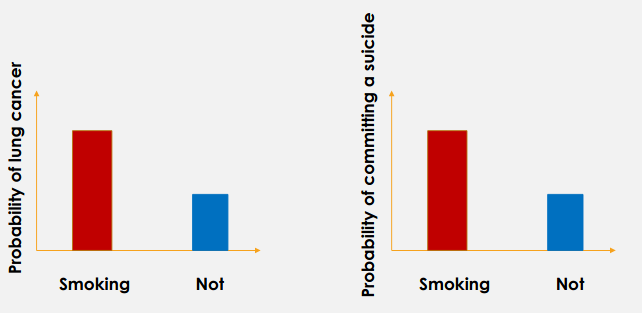
\includegraphics[width = 0.7\textwidth]{exp-design/observational.png}
\caption{Smoking and suicide: correlation not causation}
\end{figure}
Improvements that make the case for causation stronger
\begin{itemize}
\item Findinga strong correlation
\item In multiple studies using variable subjects
\item Dosage effect: mores moking leads to more cancer
\item Contrasting groups that are matched by all other variables than the one in question
\item A theory on causality
\end{itemize}

To truly prove causation, an experimental study is (probably) needed

\subsubsection{experimental, manipulative}
can \textit{determine} causality in an association. the researcher does not assign the individuals (measure plants in nature, size is not determined by the researcher).\par 
Example above: maybe use an animal experiment? That can be carried out experimentally.\par 
\noindent
\textbf{design of a manipulative experiment:} Includes a set of treatments selected for comparison. Specifies the subjects to which the treatments will be applied and gives the rules by which the treatments are allocated to the experimental units. It indicates both the measurements to be made and the analysis to be done to meet the objectives.\par 

\subsubsection{objectives in a study design}
Essential in both observational and manipulative studies.\par 
Measurements need to be accurate (free from bias of confounding variables and observer biases, expectation of random sampling and independence of replication). The measurements also need to be precise, this means reduce the influence of sampling error without risking accuracy.
\begin{figure}[h]
\centering
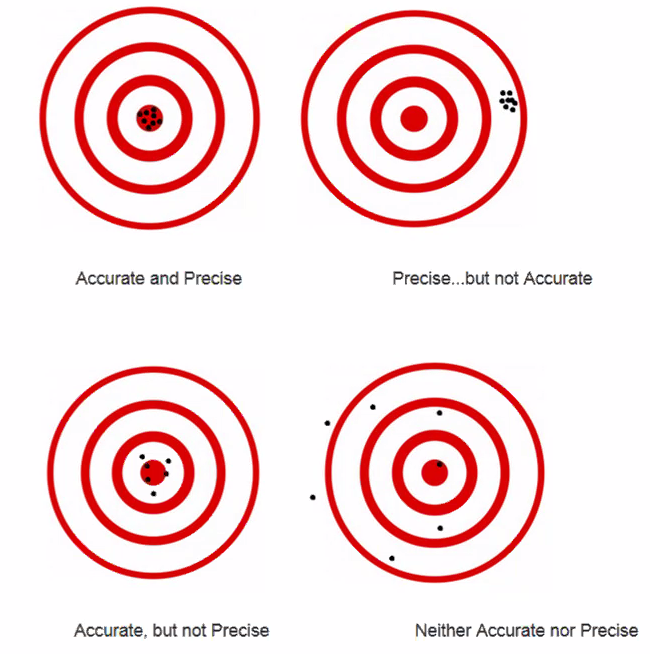
\includegraphics[width = 0.5\textwidth]{exp-design/accuratevsprecise.png}
\caption{accuracy vs. precision}
\end{figure}

\subsection{Bias}
The consistend deviaiton of estimates from the 'true' population characteristic.
One reason for bias might be confounding factors:
\begin{itemize}
\item A third, unmeasured, variable driving a correlation between variables that are not causally related
	\begin{itemize}
	\item Can be a big problem in observational studies
	\item Experimental artefacts e.g. due to sampling bias
	\end{itemize}
\item Treatments confounded in time and space (can be a problem in all kinds of studies)
\item Sampling confounded due to observer/subject unconscious biases (humans)
\end{itemize}

\subsubsection{Bias in who is being sampled}
Sampling Bias due to innate properties of subjects, unknown to the experimenter (some types of animals or people are easier to catch than others). The sampling methods themselves can also be biased (certan molecular methods are more effective for one variation of the phenomenon to be observed)

\subsubsection{Observer/Subject biases}
\begin{itemize}
\item In human studies, study subjects cause bias (placebo effect)
\item Handling in subjects in different treatment groups is biased
\item observations themselves become biased due to the observer biases
\end{itemize}
This Bias can be reduced:
\begin{itemize}
\item Blinding prevents subjects and researchers from changing their behaviour
	\begin{itemize}
	\item single blind experiment (subjects are unaware of their treatment (necessary in human studies)
	\item double blind experiment (experimenter is onaware of which treatment is applied on which subjects)
	\end{itemize}
\end{itemize}

\subsubsection{Control treatment}
The most important way to reduce bias. Treatment and control groups should be treated the same in all other ways except for the part under investigation (inactive treatment to control for placebo effect, 'sham' operations also for animal subjects, similar handling stress to subjects or disturbance caused by applying a treatment per se. \par 
In observational studies, a control group can be an age/sex/genotype matched group of individuals.
\begin{center}
\textit{no control, no conclusion!}
\end{center}

\subsubsection{Requirement of random sampling}
\begin{figure}[h]
\centering
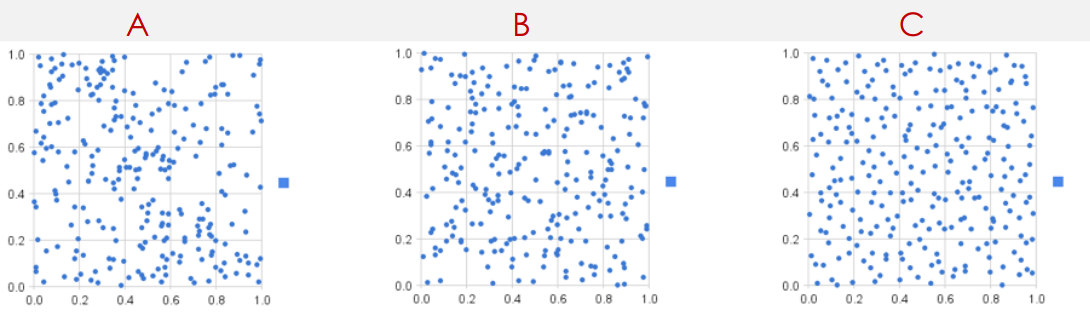
\includegraphics[width = 0.8\textwidth]{exp-design/random-sampling.png}
\caption{A: a uniform random sample of 250 points on the unit square. B: the grid is divided into the 25 squares, 10 points are randomly sampled in each smaller square. C: same as B with 64 squares with 4 randomly sampled points in each small grid}
\end{figure}
True randomness consists of a mixture of clumps and non-clumps. Randomness is different from homogeneity.\par 
in a \textit{random sample} each member of a population has an equal and independent chance of being selected. It minimizes bias and makes it possible to measure the amount of sampling error. Randomizaiton allows the later use of probability theory, and so gives a solid foundation for statistical analysis.\par 
Experimental subjects (units) should be randomly assigned to treatment groups. The aim is to randomize explicitly (use a computer, coins, dice etc.) 
\subsubsection{Precision}
The closeness whith which results of replicates in a sample agree. It is a measure of dispersion of scattering around the mean value. \par 
It is achieved through uniform experimental units, careful conduct of all operations before and during the experiment. More replicatoin also helps because it reduces the effect of chance.\par
\textbf{reduces sampling error}

\subsubsection{Replication}
The sampling error is the quantified uncertainty. A statement is of no value without a statement of uncertainty in the estimate. It allows interpolationg patterns to a whole population. It minimizes the risk of confounding effects and uncontrolled variation
\begin{figure}[H]
\centering
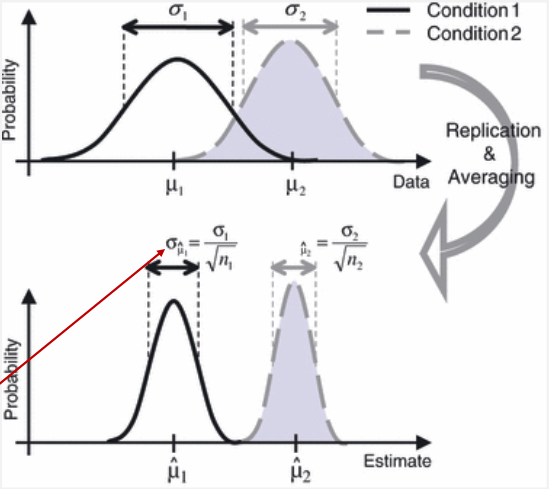
\includegraphics[width = 0.45\textwidth]{exp-design/replication.png}
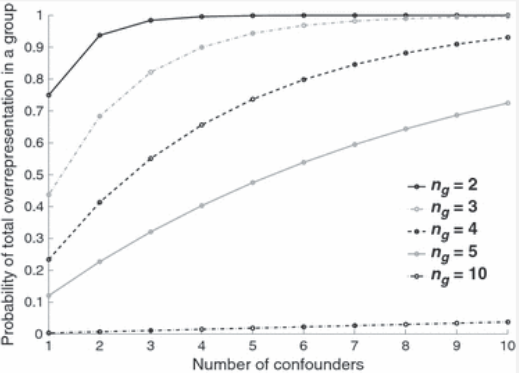
\includegraphics[width = 0.45\textwidth]{exp-design/replication2.png}
\caption{red arrow: standard error}
\end{figure}

\textbf{Problems with a small n:} \\
low statistical power, inflated false discovery rate, inflated effect size estimation, and most importantly, low reproducibility!

\begin{figure}[H]
\centering
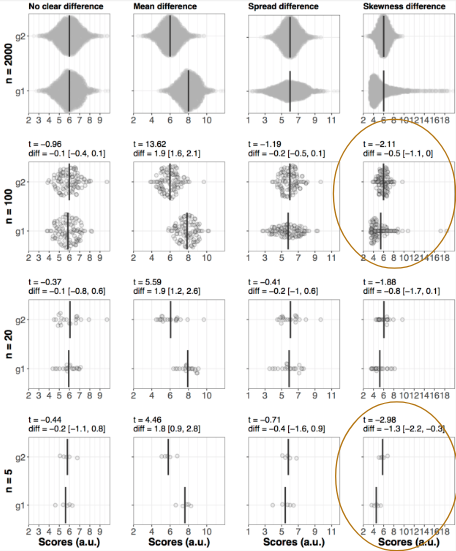
\includegraphics[width = 0.5\textwidth]{exp-design/small-n.png}
\caption{At n = 100: differnce between means -0.5. n = 5: difference in means -1.3, here the data skewness is most problematic.}
\end{figure}

Replicaiton must be \textbf{independent}, this means that every treatment must be applied to multiple independent experimental units, not just the number of units used! See Figure \ref{flowers} with different flower configurations in different chambers.
\begin{figure}[H]
\centering
\label{flowers}
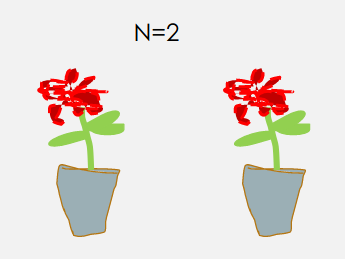
\includegraphics[width = 0.2\textwidth]{exp-design/replicationplant.png}
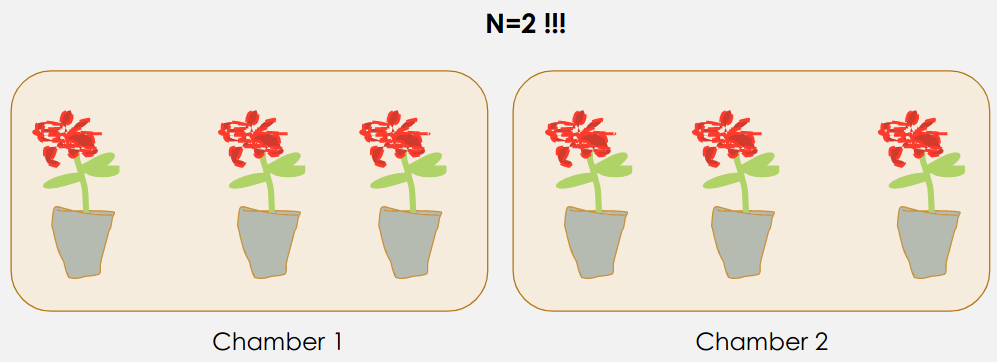
\includegraphics[width = 0.75\textwidth]{exp-design/replicationplants2.png}
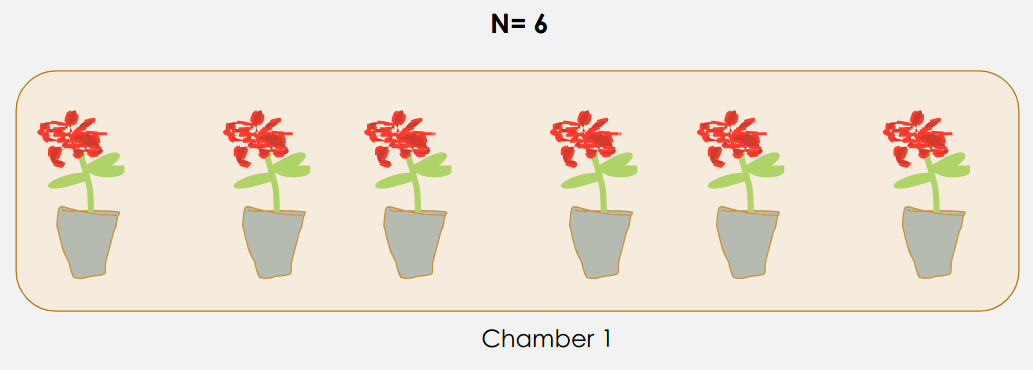
\includegraphics[width = 0.8\textwidth]{exp-design/replicationplants6.png}
\caption{n in different configurations of experiments with flowers growing in different chambers.}
\end{figure}

\textbf{Pseudoreplication} \\
This occurs whenever individual measurements are not independent but are analyzed as if they are independent of one another. Non-independence makes observations more similar to tone another and thus violated assumptions of most statistical models.\par 
Mixed-effect models are good for accounting for non-independence of replicates, e.g. 15 measurements from 10 diabetes patients give you 150 observations but just 10 independent subjects. This can be analyzed by fitting the patient as a random factor or using repeated measures ANOVA.\par 

\textbf{Example 1}\\
see which song a female bird prefers, a complex one or a simple one (sung by two different males). Playback each type of song to 40 females and see how they respond.\par 
This is problematic because the females might prefer one male's voice over the other instead of the complexity ($\rightarrow$ get multiple complex/simple songs from different males)\par 
\vspace{0.35cm}
\noindent
Good experiments are comparative (compare to control group, replicate to rule out significant effects occuring only by chance).\\
Be aware of bias (are genotypes different...)\\
Generalize the experiment (plant growth not only at 20 and 25 degrees, but more steps and higher range, take different genotypes into accound...)\\

\subsection{Stratification or 'Blocking'}
Grouping of experimental units that have similar properties. Whithing each block, treatments are randomly assigned to experimental units. Ised to account for extraneous variation by dividing the experimental units into groups (called blocks or strata) that share common features. Essentially repeats the same completely randomized experiment several times (treatment effects analyzed whithin each block).\par 
A block can be:
\begin{itemize}
\item Field plots experiencing similar local conditions
\item animals from the same litter
\item Patients attending the same clinic
\item Runs of an experiment executed on the same day
\item illuma lanes on which samples are sequenced
\end{itemize}
Example:
The greenhouse fits too few plants for a a large scale experiment, multiples sets have to be measured over 6 months to get a high enough replication.
\begin{figure}[H]
\centering
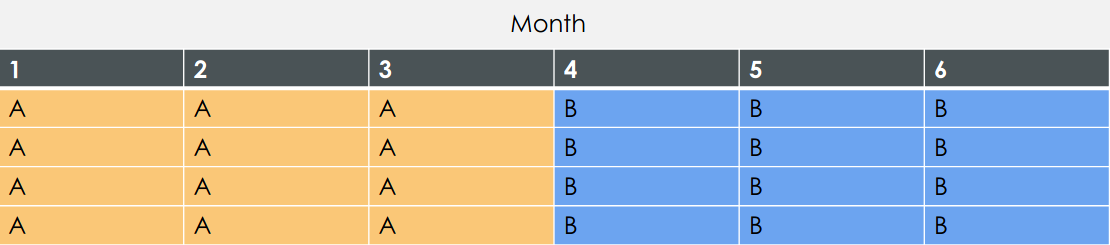
\includegraphics[width = 0.9\textwidth]{exp-design/greenhouse1.png}
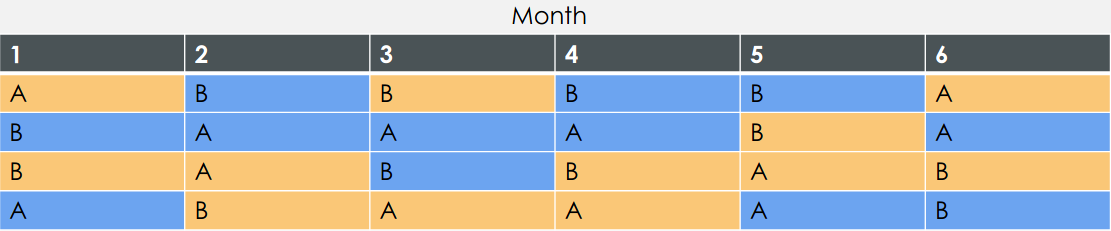
\includegraphics[width = 0.9\textwidth]{exp-design/greenhouse2.png}
\caption{A, B = genotypes, blue = 20C, orange = 25C. First image: confounding variables of month and genotype. Can be solged by 2: randomized block design. Month is now a blocking factor $\rightarrow$ the whole experiment is now replicated within each month. Genotype and temperature factors are balanced within each month.}
\end{figure}

\subsubsection{Randomizing and blocking}
It is bestito fix a variable if possible. e.g. use a single genotype if individual variation is to be minimized. If that is not possible, block (see months above). If that is not possible, randomize. A block needs to be recorded and accounted for in a model!\par 

\subsubsection{Aim for a balanced design}
A design is balanced when there are equal numbers of replicates at all levels of all conditions. The second major way to reduce the influence of sampling error on estimation and hypothesis testing. SE \textcolor{red}{what does that stand for?} of the differences between the means is smalles when ($1/n_1 + 1/n_2$)is smallest
\begin{equation*}
\begin{split}
& n_1 = n_2 = 10 \;\;\; \Rightarrow \;\;\; ( \frac{1}{10} +\frac{1}{10} ) = 0.2 \\
& n_1 = 19,\; n_2 = 1 \;\;\; \Rightarrow \;\;\;(\frac{1}{19} + \frac{1}{1})= 1.05
\end{split}
\end{equation*}
This helps with robustnes against assumptions about the distributions of the populations. Problems with non-normality and unequal variabces matter less with balanced designs.


\subsubsection{Factorial designs}
Investigates all treatment combinations of two or more variables. When we are interested in effects of multiple treatments, or factors, and their interactive effects, for example genotype-by-environment interactions

\subsection{Summary}
Experiments need to be designed well in order to eliminate bias and reduce sampling error when estimating the effects of one variable on another. Good design and good analyssis can lead to reduced samle sizes (saves money, time and \textit{animal lives})


\subsection{practical application lab 6}
install the \texttt{BiocManager} package to install \texttt{EdgeR, baySeq}.
\begin{lstlisting}
if (!requireNamespace("BiocManager", quietly = TRUE))
	install.packages("BiocManager")

BiocManager::install()
BiocManager::install(c("edgeR","baySeq"))
library(baySeq)
library(edgeR)
\end{lstlisting}
load data set 
\begin{lstlisting}
load("mobData.RData")
head(mobData)
mobDataGroups<-c("MM","MM","WM","WM","WW","WW") #M = mutated, W=wildtype
 # Make a vector that gives a name to the treatments. This is needed to identify the treatment groups in the expression dataset.
\end{lstlisting}
Make \texttt{d} a DGEList, \texttt{d\$counts} is a table of integer read counts, with rows corresponding to genes and columns to independent libraries, which edgeR can use.\par 
\begin{lstlisting}
d<-DGEList(counts=mobData,group=factor(mobDataGroups)) 
\end{lstlisting}
the groups/libraries and their information is stored in \texttt{d\$samples}\\
\textbf{Filtering the data}\\
look at counts per million (normalize each library to 1 mil. expressions in total
\begin{lstlisting}
d.full<-d
head(cpm(d)) #cpm = counts per million
apply(d$counts,2,sum)# Total counts per sample
keep<-rowSums(cpm(d)>100)>=2 # Specify rows thatmeet our filtering criteriad<-d[keep,] # usually 1, not 100
d$samples$lib.size<-colSums(d$counts)# Re-compute the library size since now they have fewer tags.
dim(d.full) 
	[1] 3000   6
dim(d)
	[1] 724   6
\end{lstlisting}

minimize difference between the libraries, so that any remaining differences are truly biological and not jost technical.

\begin{lstlisting}
d<-calcNormFactors(d)#Without this, the default value is 1 for all values in d$samples$norm.factors.

plotMDS(d,method="bcv",col=as.numeric(d$samples$group))
legend("bottomleft",as.character(unique(d$samples$group)),col=1:3,pch=20)
\end{lstlisting}

\begin{figure}
\centering
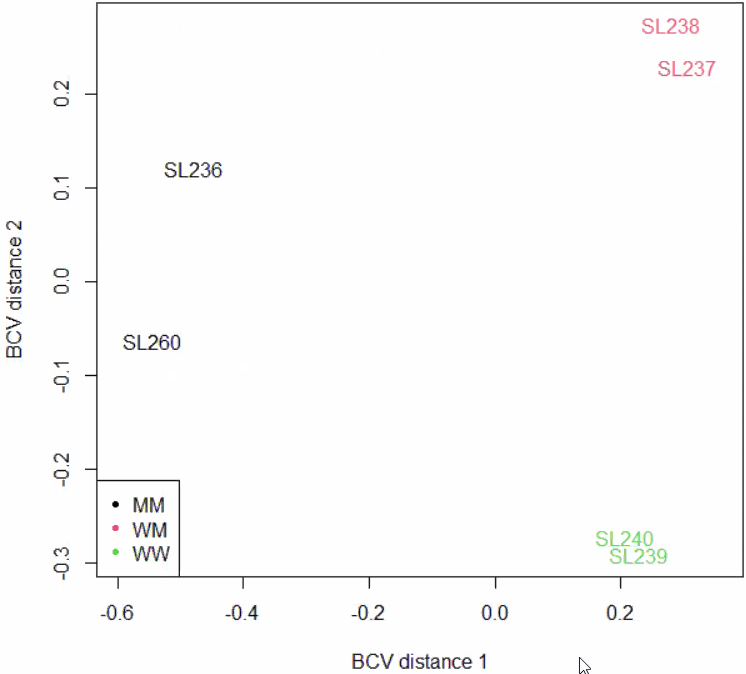
\includegraphics[width= 0.5\textwidth]{lab6-exp-design/mdsplot.png}
\end{figure}



\vfill

\section{Genome Wide association studies (GWAS), ways to control for multiple testing}
\subsection{association mapping}
Associate a Phenotype to a position in the genome. This can be accomplished with the help of:
\begin{itemize}
\item SNPs: single nucleotid polymorphism (most of the time)
\item Insertions or deletions 
\item CNVs: copy number variations
\item Epigeneitc markers
\end{itemize}
These variations can be used to tie the genetic marker to a phenotype variation. Identifying large amounts of associations efficiently is a problem, but necessary.

\subsection{Quantitative traits}
Assuming the Phenotype is quantitative and additive, it can be modeled as a linear regression model with the sum over the predicted variables:
\begin{equation*}
y_i \;\; = \;\; \beta_0 + \sum^m_{j=1} x_{i, j} \; \beta _i +\epsilon_i
\end{equation*}
assume we analyze a SNP dataset, where each sequence is associated with its phenotype (the genotypes are assued to be fixed)
\begin{itemize}
\item $y_i$ is the phenotype of the $i^{th}$ individual (dependent variable)
\item $\beta _0$ is the mean/intercept
\item $x_{i,j}$ is the genotype of the $i^{th}$ individual and the $j^{th}$ SNP variant
\item $\beta_j$ is the effect size of the $j^{th}$ variant (estimated regression coefficient)
\item $\epsilon_i$ is the error or noise term of the $i^{th}$ individual (usually assumed to be independent and gaussian distributed.
\end{itemize}
A t-test can be used to test whether there is a significant effect. (an equivalent F-test is also possible)
\begin{equation*}
t = \frac{\hat{\beta}_j}{S E _{\hat{\beta}_j}} \;\;\; where \;\;\; \hat{\beta}_j = \frac{\sum^n _{i=1} x_{ij} \; y_i}{\sum^n _{i=1} x_{ij}^2}
\end{equation*}

$\hat{\beta}_j$ is the regression coefficient, aka the least square estimate (the result of the linear regression where sums of squares is to be minimized). $t$ is here basically the regression coeffitient $\hat{\beta}_j$ divided by the standard of that regression coefficient $SE_{\hat{\beta}_j}$.\par 
Effects of other markers are explicitely ignore. Most GWAS for quantitative traits are conducted using this (or an equivalent) statistic.\par 

With a t-test statistic we can obtain the p-value (the probability that $t$  or a more extreme value is observed under the null hypothesis ($H_0$ is that the marker has no effect, which means that $\beta_j = 0$)
\begin{equation*}
P(T \geq t|H_0) = p-value
\end{equation*}

\subsection{principle of an association study}
\textbf{example} Measure phenotypes of flowers and sequence their SNPs (four different ones here)
\begin{table}[H]
\centering
\caption{0 = homocygous (homozygot) for the most common allele, 1 = heterocygous for the more and less common allele, 2 = homocygous for the rare allele.}
\begin{tabular}{c|c|c|c|c|c}
& number of flowers & SNP1 & SNP 2 & SNP 3 & SNP 4 \\
\hline
A1 & 8 & 1 & 2 & 0 & 1 \\
\hline 
A2 & 9 & 1 & 0 & 0 & 2 \\
\hline
A3 & 12 & 2 & 2 & 2 & 1 \\
\hline 
A4 & 6 & 0 & 1 & 1 & 0 \\ 
\hline
A5 & 17 & 2 & 2 & 1 & 1 \\
\hline
A6 & 4 & 0 & 2 & 2 & 1 
\end{tabular}
\end{table}
Do some of the slips associate with the number of flowers the plant produces? use a linear regression framework: the genotype is the dependant variable.

\begin{figure}[H]
\centering
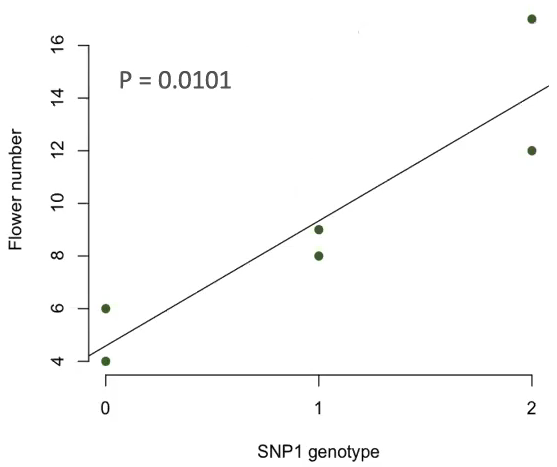
\includegraphics[width = 0.6\textwidth]{gwa/arabidopsis-lm.png}
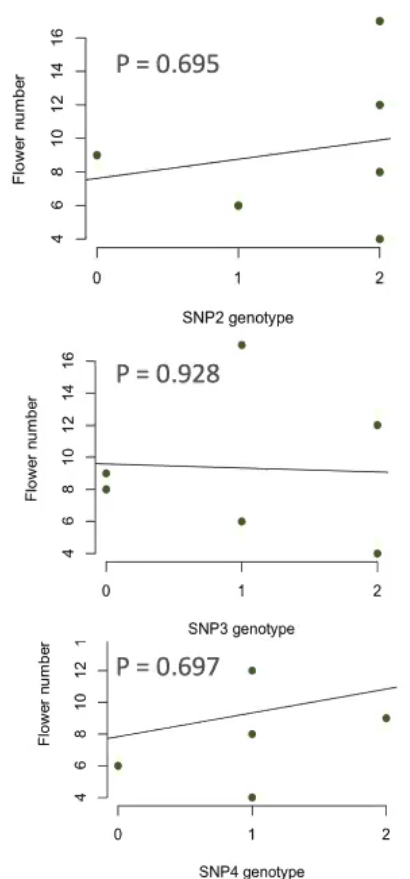
\includegraphics[width = 0.29\textwidth]{gwa/arabidopsis-lm2.png}
\caption{linear model with flower number and SNPs. for SNP1 there seems to be a more significant statistic association than for the others}
\end{figure}

Usually there are way more than 4 tests, this means that the model needs to be corrected for multiple testing. a 5\% significance threshold ($\alpha$) is used.

\subsubsection{Bonferroni correction}
assume that each locus/marker is independent from all others. A conservative bound on the probability of rejecting the null hypothesis for rejecting one or more markers for a given significance threshold $\alpha$.
\begin{equation*}
1-P(T_1 \leq t, ..., T_m \leq t|H_0) \leq \alpha
\end{equation*}


\subsubsection{Family wise error rate (FWER)}

\renewcommand{\arraystretch}{1.75}
\begin{table}[H]
\centering
\caption{Truth vs. significant and non-significant effects and second table for multiple hypothesis tests. R is the total number of significant tests, m is the total number of all tests. $m_0$ is the number of true null-hypothesis tests.}
\begin{tabular}{c|c|c}
Truth & Non-significant & Significant \\
\hline
$H_0$ & True negative (U) & Type I error (V) \\
\hline 
$H_A$ &Type II error (T) & True positive (S)
\end{tabular}
\begin{tabular}{c c}
                             \hspace{10cm}    &                                            
\end{tabular}

\begin{tabular}{c|c|c|c}
Truth & Non-significant & Significant \\
\hline
$H_0$ & U & V & $m_0$ \\
\hline 
$H_A$ &T & S & $m-m_0$ \\
\hline 
& m-R & R &m

\end{tabular}
\end{table}
\renewcommand{\arraystretch}{1}

The Family wise error rate is the probability of at least one type I error (V) $FWER = P(v \geq 1)$.
There are two controls of the FWER 
\begin{itemize}
\item assuming that all $H_0$ are true, control the complete error rate $FWEc(complete \; null) = P(V \leq 1 |H_0 ^c true) $ which assumes $H_0 ^c = [H_0 ^1, H_0^2, ..., H_0 ^m]$
\item control the partial FWER $FWEc(partial \; null) = P(V \leq 1 |H_0 ^c true) $
\end{itemize}
This allows for stronger or weaker controls.\par 
If there are $m = 2$ tests with two null-hypotheses $H_0 ^1, H_0^2$, there are four partial null scenarios: both $H_0$ are true, only one of them is, or none is. if the FWER is to be controlled, this means that the type-I error rate is to be controlled.

\subsubsection{False discovery rate}

See second table in FWER (errors for multiple Hypothesis tests). Here the fraction of Type I errors out of the total number of significant discoveries. an expected rate of false positives. $$FDR = E\left( \frac{V}{R}\right) $$
Only if all null-hypothesis are true, this is equal to the FWER (otherwise not!). As false positives increas, true positive will also increase.

Control for the FDR through the Benjamini Hochberg procedure (B-H Procedure):
\begin{itemize}
\item The p-values are obtaines and ordered $$p_{(1)} \leq ... \leq p_{(m)}$$ with the corresponding null hypotheses $H_0^{(1)} , ..., H_0^{(m)}$.
\item k (critical number by which the hypotheses are rejected) is defined as follows: 
\begin{equation*}
k = \max \Big\{ i: p_{(i)} \leq \frac{i}{m}q \Big\}
\end{equation*}
each p-value is compared, find the threshold of p-values $p_{(k)}$ where it is just smaller than $\frac{i}{m}q$. each null hypothesis $H_0^{(1)} , ..., H_0^{(k)}$ can then be rejected.
\end{itemize}

\subsubsection{Example}
\textbf{Bonferroni correction in practice:} $m = 10$, $\alpha = 0.05$ \\
estimate FWEC: $$1-(1-\alpha)^m \; = \; 0.4$$
Not controlling the FWER on 10 tests gives a 40\% error rate. should be lower! This can be corrected by using $\frac{a}{m}$ instead of $\alpha$, which gives $$1-(1-\alpha)^{\alpha/m} \; = \; 0.4$$
The FWER is much smaller now, The bonferroni corrections lets us correct the FWER at a specified $\alpha$.

\noindent
\textbf{FDR correction in practice (B-H):}\\
\begin{table}[H]
\centering
\caption{p-values and the t-value vector from the false discovery rate $\frac{i}{m}q$.}
\begin{tabular}{c|c}
p-values & 0.001 0.012 0.014 0.122 0.245 0.320 0.550 0.776 0.840 0.995\\
\hline
t-calculation & 0.005 0.010 0.015 0.020 0.025 0.030 0.035 0.040 0.045 0.050\\
\end{tabular}
\end{table}
For the comparison (see FDR equation) a new $\alpha = 0.05 \frac{i}{10}$ value is used. This means k = 3 since $p_{(3)} = 0.014 \leq 0.015$, so $H_0^{(1)} , H_0^{(2)},  H_0^{(3)}$ can be rejected. Even though the p-value of the second one is lower than the corrected alpha. For the Bonferroni correction only $H_0^{(1)}$ would be rejected.

Which correction should be used?\\
Depends on the question and the data: drug development is very strict -> needs very low Type-I error. 

\subsubsection{Using the Association mapping}
in reality, a lot of SNPs are tested, but you cant show so many regression plots. The outcome is visualized with manhattan plots.
\begin{figure}[H]
\centering
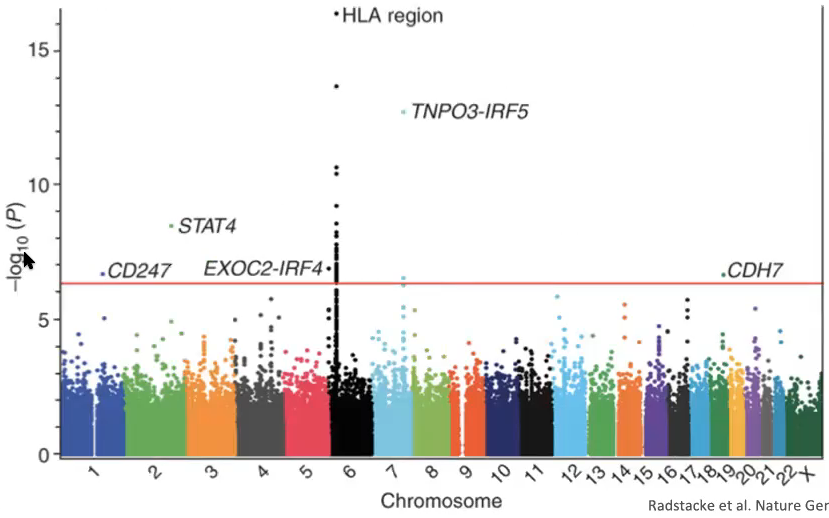
\includegraphics[width = 0.7\textwidth]{gwa/manhattan.png}
\caption{Manhattan plot. Each point is the p-value from a linear regression. Higher on the axis the smaller is the p-value (the higher the association). The red line is the genome-wide significance threshold (can be obtained through controlling the FWER or FDR)}
\end{figure}
The next step would be to look up which genes are on the places with significance.

\subsection{Linkage disequilibrium (LD)}
Not the whole genome is available, it is very unlikely that the Causative locus is actually in the subsample that was evaluated.

\begin{figure}[H]
\centering
\includegraphics[width = 0.6\textwidth]{gwa/linkage-equilibrium.png}
\caption{visualization of how the correlation between the marker locus in the subsample and the phenotype can occur.}
\end{figure}
How strong is the correlation between the Typed marker locus and the causative locus (so called linkage disequilibrium)? This makes it possible to detect the indirect association. Neighbouring markers (physical closeness) will likely be inherited together, causing linkage disequilibrium (LD) between the two markers. 

\begin{figure}[H]
\centering
\includegraphics[width = 0.5\textwidth]{gwa/ld-plot.png}
\caption{Linkage Disequilibrium plot, see cursor, region of very high LD. LD can also extend across chromosomes (see enlarged area)}
\end{figure}
The LD stucture of the genome is useful, because you don't have to tag every SNP, it is possible to design SNPs that tag the structure of larger haplotype blocks (because many snips in e.g. the red area would be redundant, you don't need many SNPs to describe the variation/change).

\subsection{confounding in GWAS}
Confounding factors can influence the result and can be controlled for.
\subsubsection{population structure}
One population lives kind of secluded in one area which leads to reduced gene-flow and can lead to differences in allele-frequencies to other populations.\\
\textbf{population:} collection of individuals (typically within a restricted geographical area) that have a non-zero probability to inbreed.\\

\LARGE{\textcolor{red}{Continue with the second recording}}

\end{document}






















